\clearpage
\section{Invariant Mass Spectra}
\label{sec:results}

The final dielectron mass spectra from data and standard model prediction are shown in Figure~\ref{mass_2016} (\ref{mass_2017}) together with the integral of the mass spectra in 2016 (2017).
The ratios of dielectron mass spectra between data and standard model prediction in signal region are shown in Figure \ref{massratio_2016} (\ref{massratio_2017}) in 2016 (2017).

The following systematic uncertainty sources are considered.

\begin{itemize}
  \item[$\bullet$] Pile up reweighting: due to the HEEP ID scale factor (see Figures \ref{fig:SS_nominal_PV_2016} and \ref{fig:SS_nominal_PV_2017}) is not flat versus pile up. Therefore, different pile up reweighting condition will give different total number of MC events. This uncertainty is considered by scaling the minimum bias cross section (which is used for producing the pile up distribution of data) up and down by 1 sigma (4.6\%).
  \item[$\bullet$] DY PDF: due to the DY mass spectrum may dependent on the choosing of PDF, the effect of using different PDFs is estimated (see Section \ref{sec:dyBkgCorr}). This uncertainty is considered by applying a mass dependent uncertainty on the DY cross section (for mass $>120$ GeV) (see Figure \ref{fig:pdf_rel_uncert}).
  \item[$\bullet$] Cross section of background processes: 7\% (around 1 sigma for \ttbar) uncertainty is considered on the cross section of the non-DY background estimated from MC for different processes.
  \item[$\bullet$] Jet background: 50\% uncertainty is considered on fake jet contribution due to the uncertainty on the fake rate estimation.
  \item[$\bullet$] Electron energy scale: From the energy scale study using boosted Z events (see Figures \ref{fig:data_MC_Et_E_BB} and \ref{fig:data_MC_Et_E_BE}), the considered uncertainty on electron energy scale for high mass region is 2\% for barrel-barrel and 1\% in barrel-endcap (for mass $>120$ GeV).
  \item[$\bullet$] HEEP ID scale factor: From the HEEP ID scale factor study (see Section \ref{sec:Zprime_SF}), one can see in low \et region the scale factor can be measured precisely, while for high \et region, due to the lack of statistics, the uncertainty on the scale factor is increased. Therefore, a \et dependent uncertainty on HEEP ID scale factor is considered. For barrel it is 1\%  below 90 GeV and 1-3\% linearly increase for 90 GeV - 1 TeV range and 3\% for higher than 1 TeV. For endcap it is 1\% below 90 GeV and 1-4\% linearly increase for 90 GeV - 300 GeV and 4\% for higher than 300 GeV in 2016. In 2017 it is the same for barrel, for endcap it is 2\% below 90 GeV and 1-5\% linearly increase for 90 GeV - 300 GeV and 5\% for higher than 300 GeV.
  \item[$\bullet$] Normalization to Z peak: As we normalized MC to data in Z peak region, there are other uncertainties (which is not mentioned above) could affect Z peak normalization like the uncertainty on trigger efficiency measurement, gsf reconstruction efficiency measurement, and DY cross section in Z peak. All these uncertainties can be merged into one uncertainty which is the Z peak normalization uncertainty. Based on the DY cross section measurement in Z peak region study (see Section \ref{sbusec:DY_xs}), the Z peak normalization uncertainty is considered as 1\% in 2016 and 2\% (4\%) for barrel-barrel (barrel-endcap) in 2017.
\end{itemize}


\begin{figure}[!htbp]
  \begin{center}
    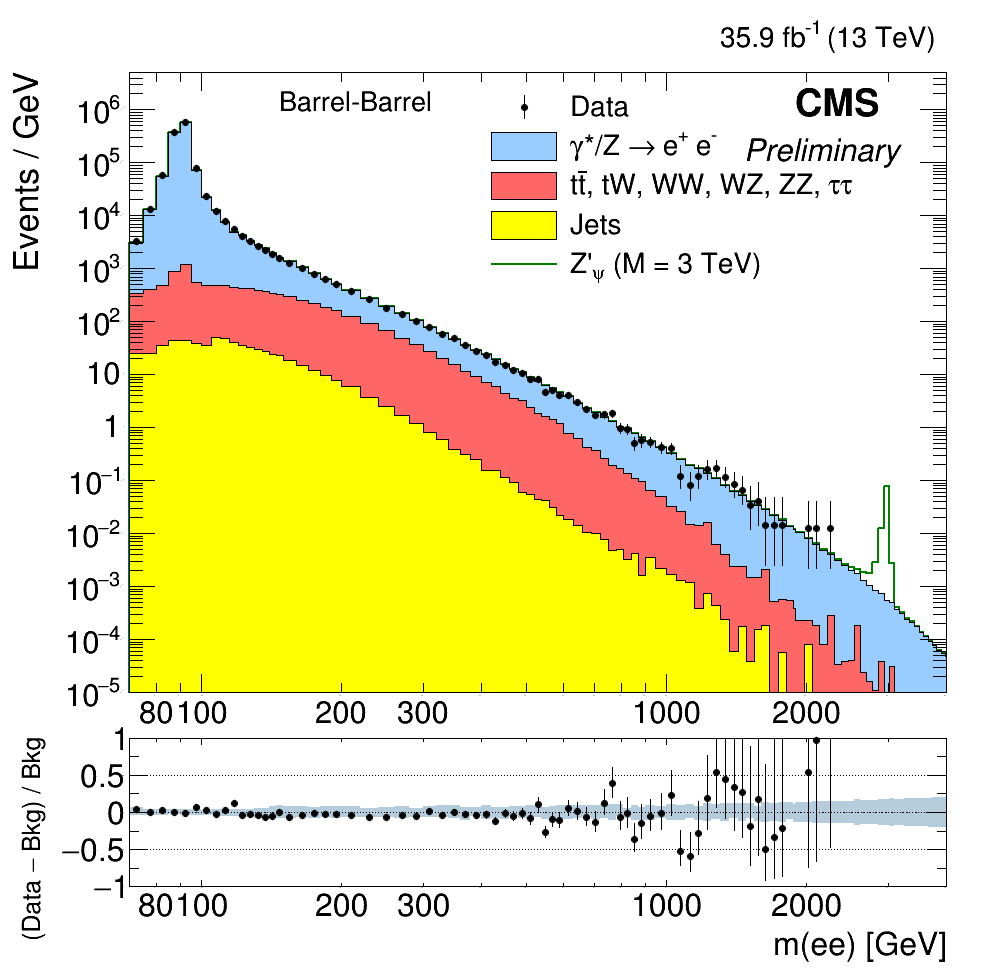
\includegraphics[width=0.47\textwidth]{figures/Zprime/2016/mass/massHistEBEB}
    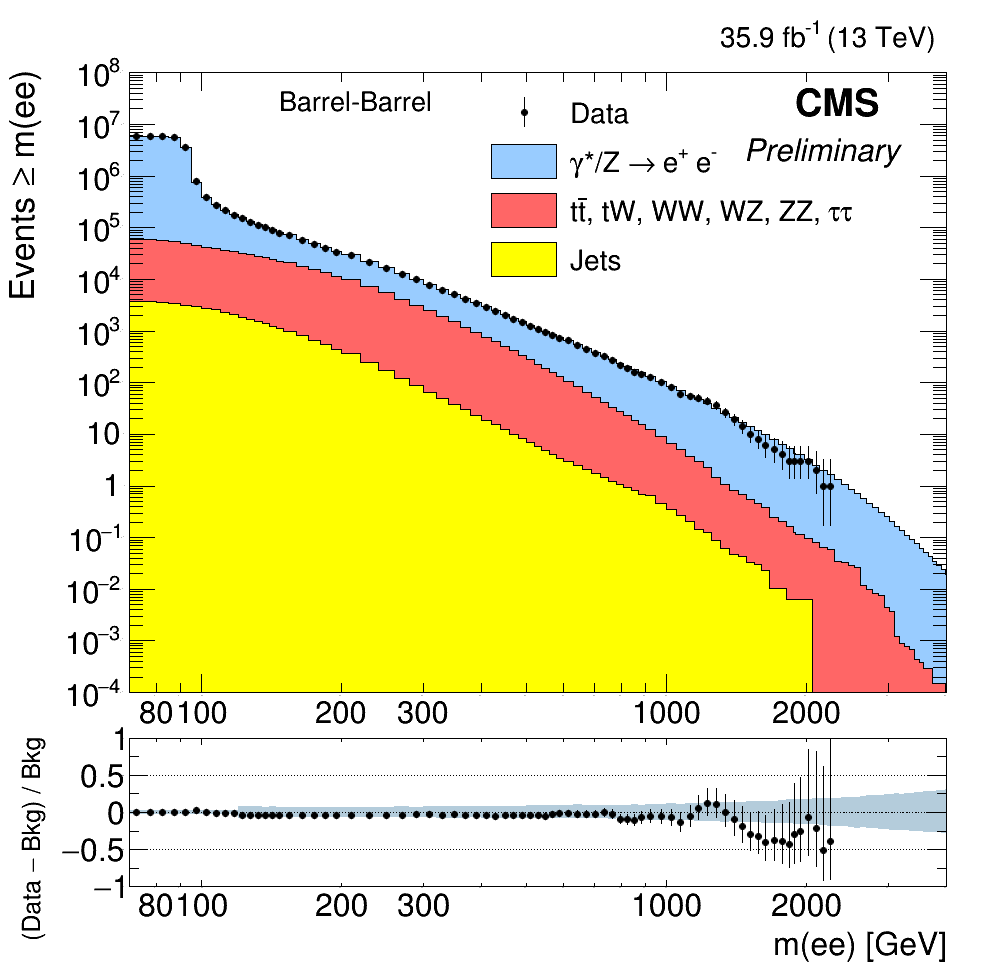
\includegraphics[width=0.47\textwidth]{figures/Zprime/2016/mass/cMassHistEBEB}
    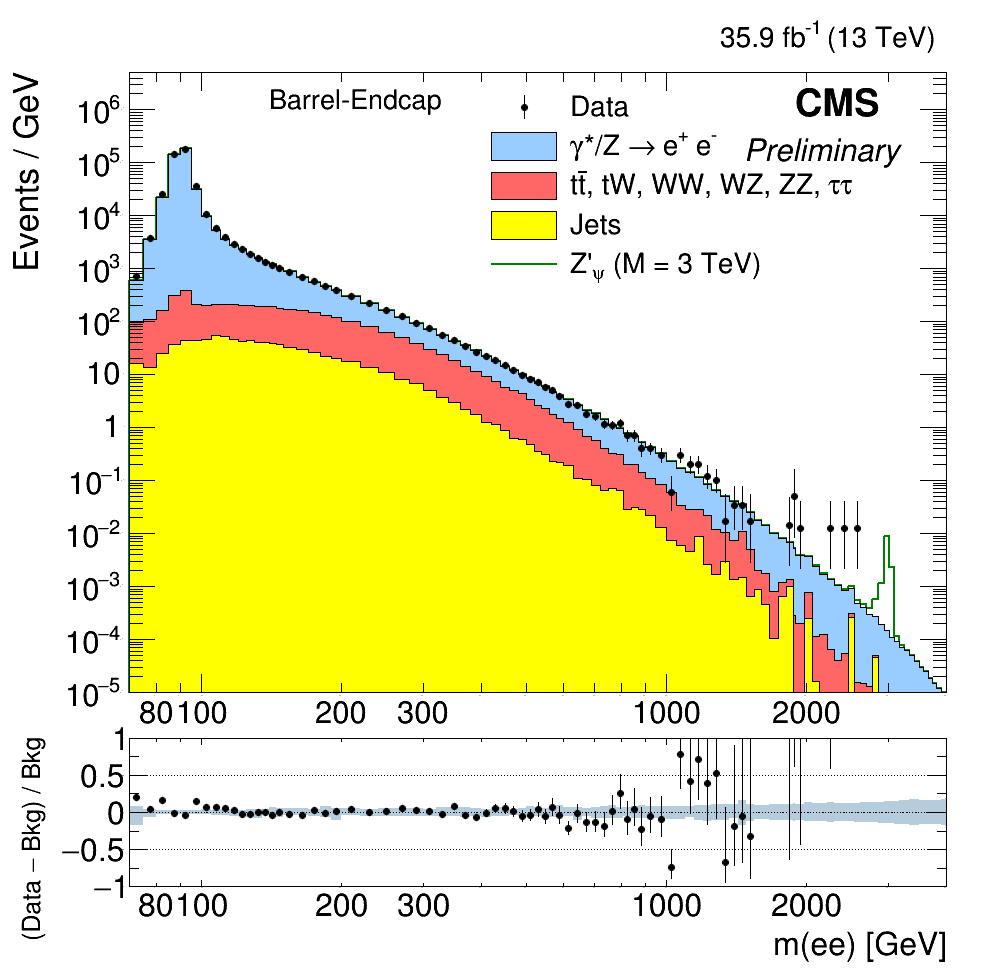
\includegraphics[width=0.47\textwidth]{figures/Zprime/2016/mass/massHistEBEE}
    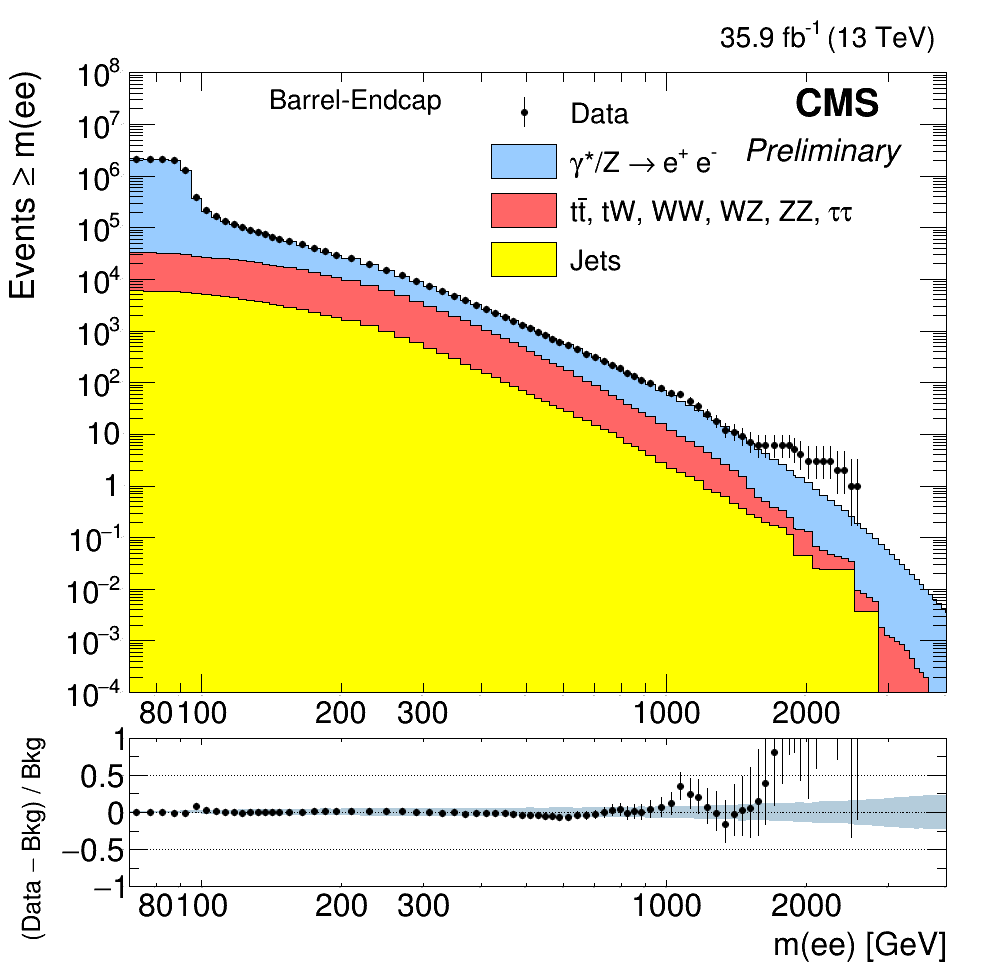
\includegraphics[width=0.47\textwidth]{figures/Zprime/2016/mass/cMassHistEBEE}
    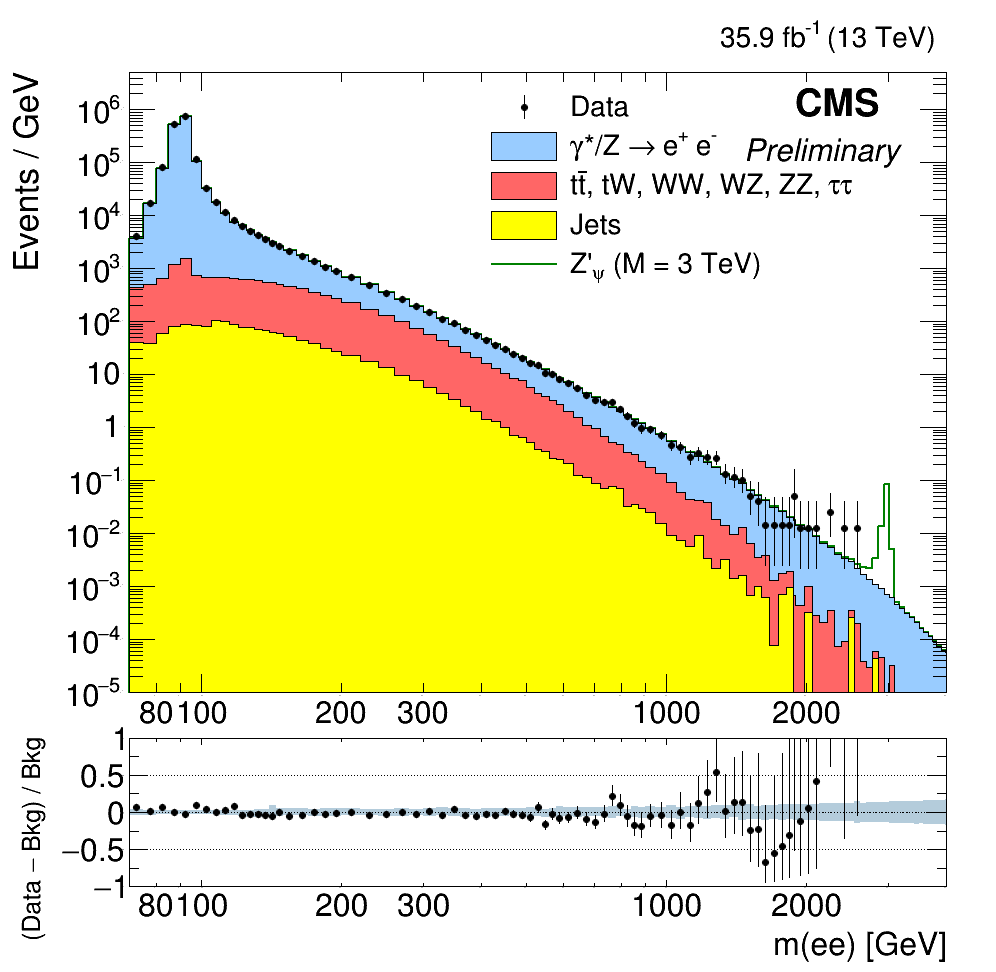
\includegraphics[width=0.47\textwidth]{figures/Zprime/2016/mass/massHist}
    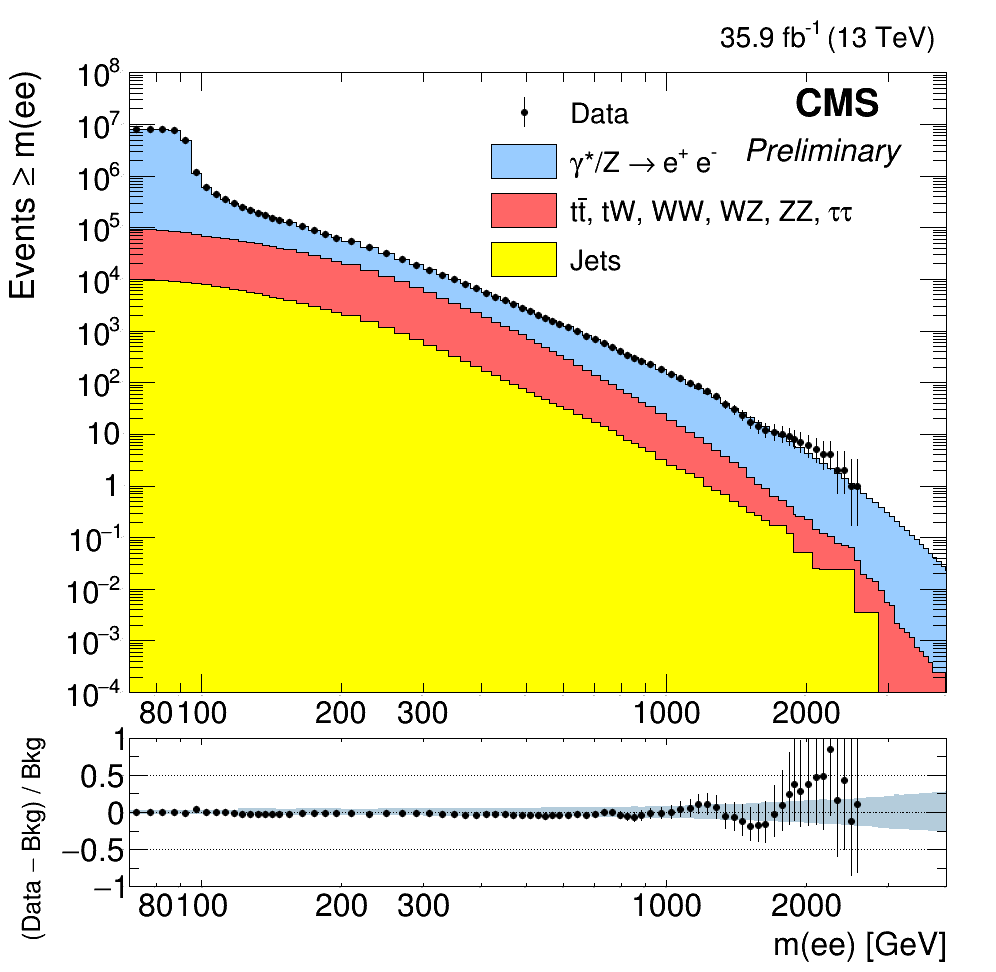
\includegraphics[width=0.47\textwidth]{figures/Zprime/2016/mass/cMassHist}
    \caption{The observed dielectron mass spectrum (left) and the integral of the measured dielectron mass spectrum (right) for barrel-barrel (top), barrel-endcap (middle) and sum of the barrel-barrel and the barrel-endcap (bottom) together with the predicted standard model backgrounds in 2016.}
    \label{mass_2016}
  \end{center}
\end{figure}

\begin{figure}[!htbp]
  \begin{center}
    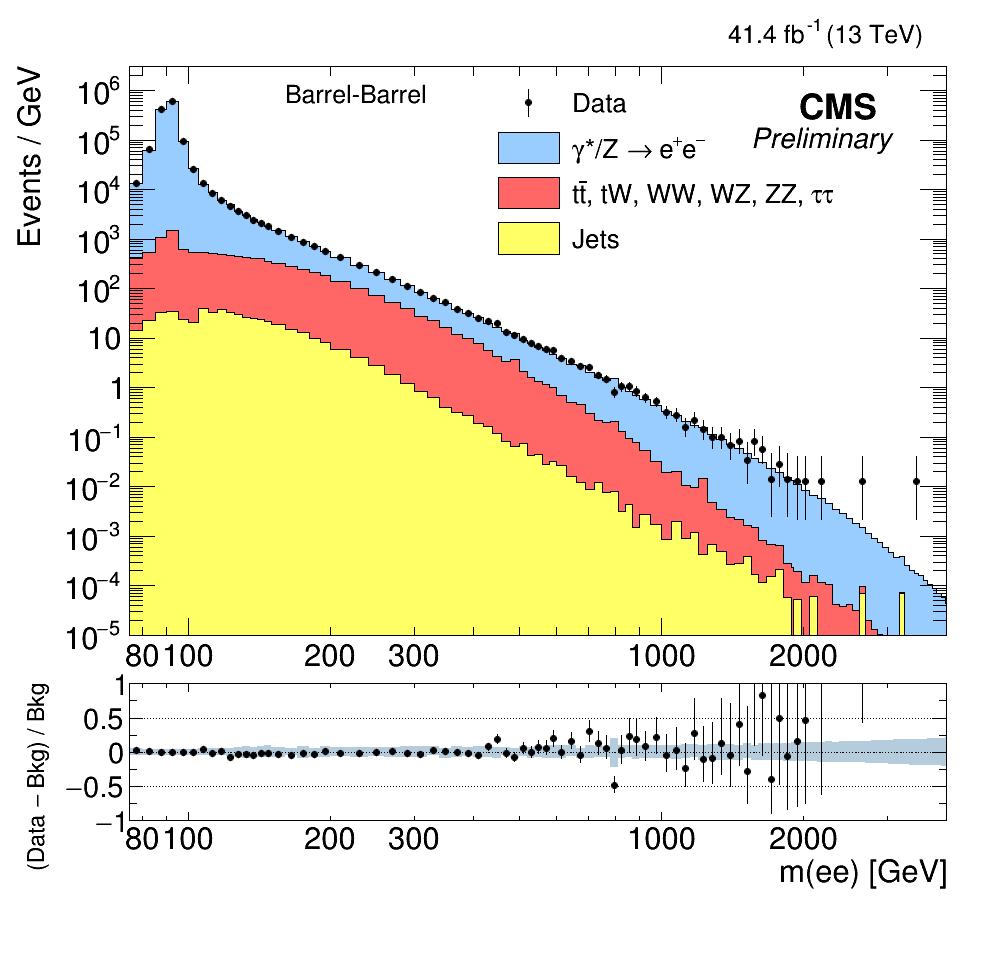
\includegraphics[width=0.47\textwidth]{figures/Zprime/2017/mass/massHistEBEB}
    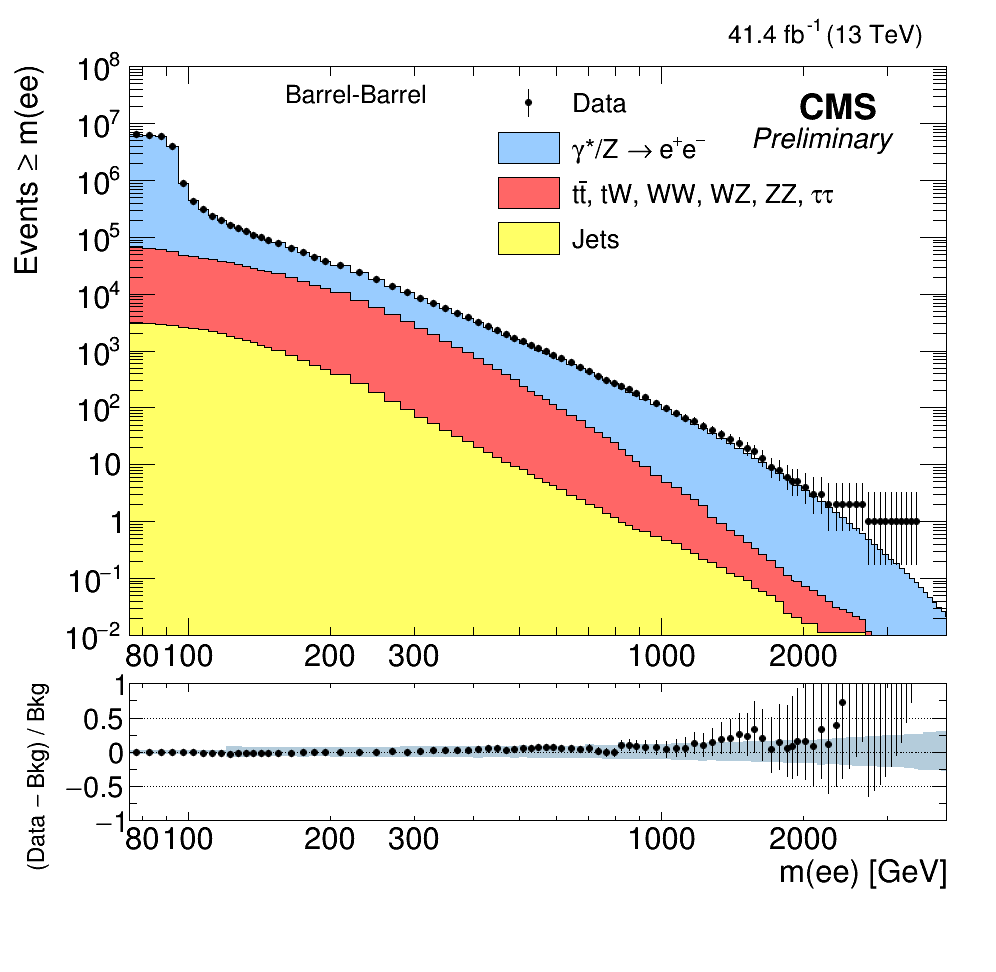
\includegraphics[width=0.47\textwidth]{figures/Zprime/2017/mass/cMassHistEBEB}
    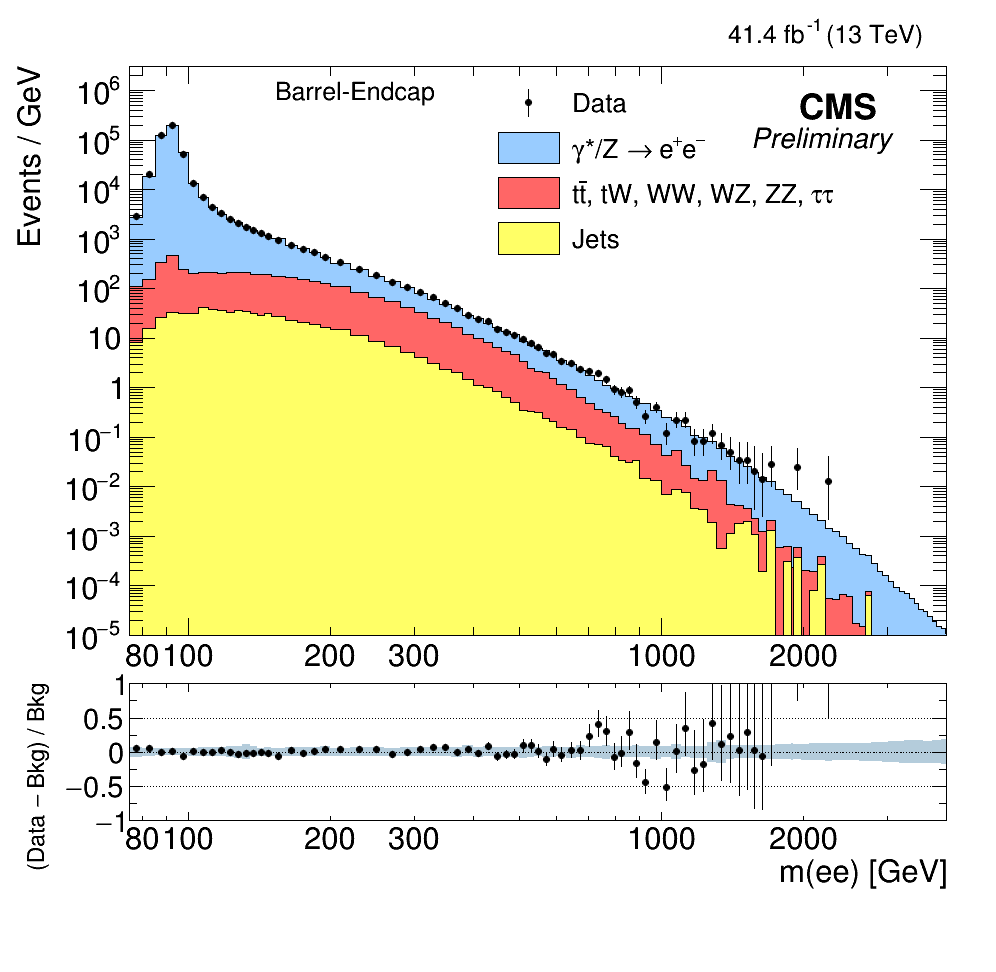
\includegraphics[width=0.47\textwidth]{figures/Zprime/2017/mass/massHistEBEE}
    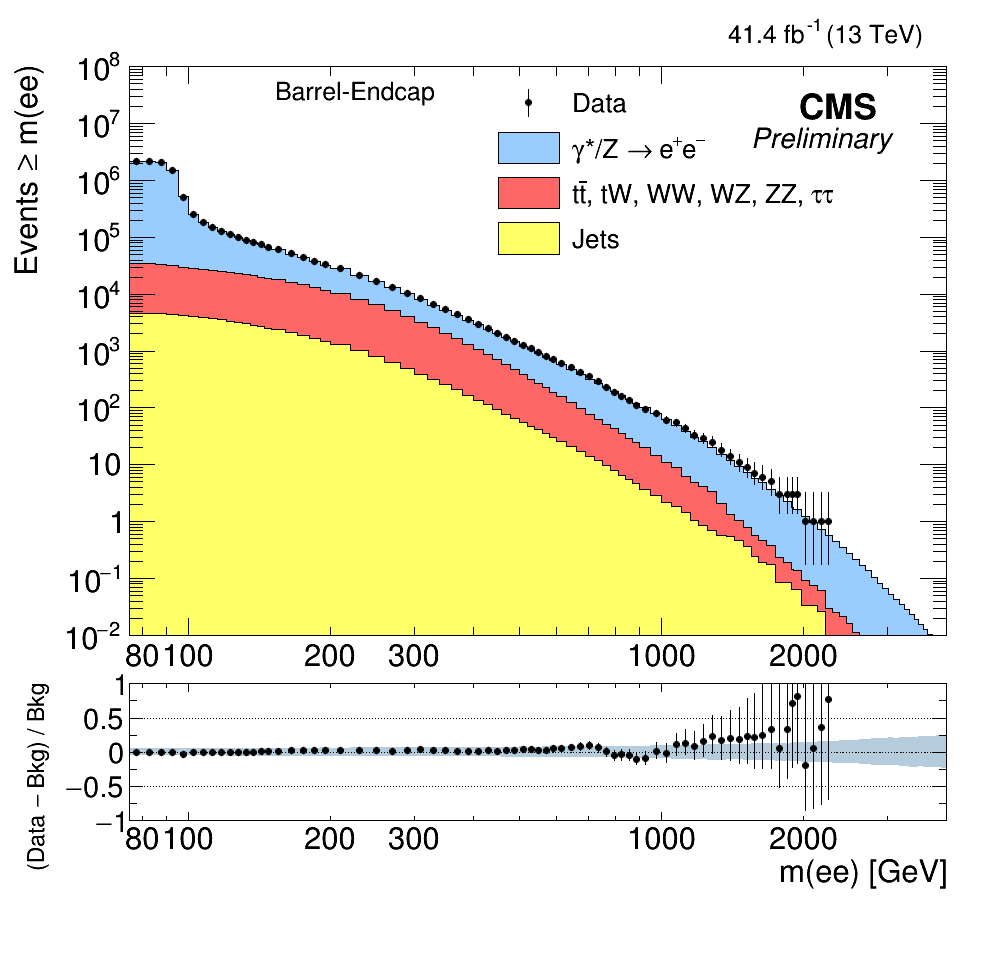
\includegraphics[width=0.47\textwidth]{figures/Zprime/2017/mass/cMassHistEBEE}
    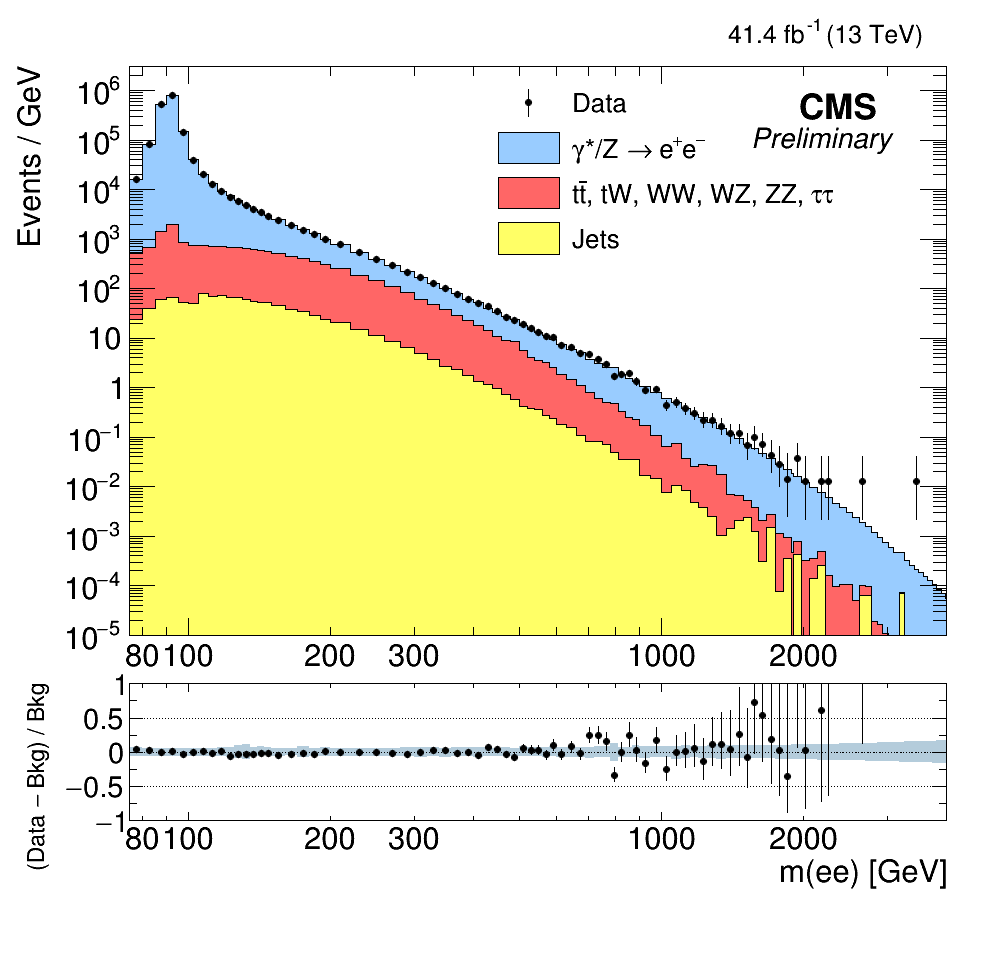
\includegraphics[width=0.47\textwidth]{figures/Zprime/2017/mass/massHist}
    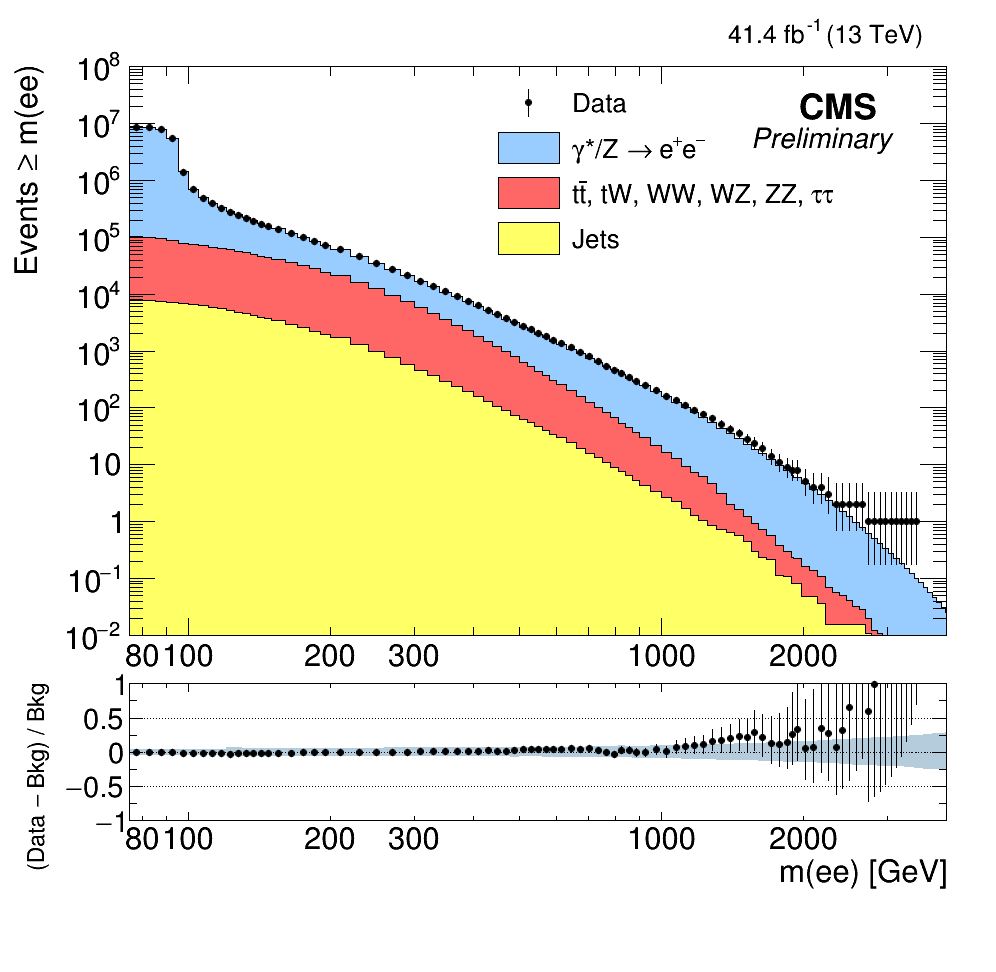
\includegraphics[width=0.47\textwidth]{figures/Zprime/2017/mass/cMassHist}
    \caption{The observed dielectron mass spectrum (left) and the integral of the measured dielectron mass spectrum (right) for barrel-barrel (top), barrel-endcap (middle) and sum of the barrel-barrel and the barrel-endcap (bottom) together with the predicted standard model backgrounds in 2017.}
    \label{mass_2017}
  \end{center}
\end{figure}

\begin{figure}[!htbp]
  \begin{center}
    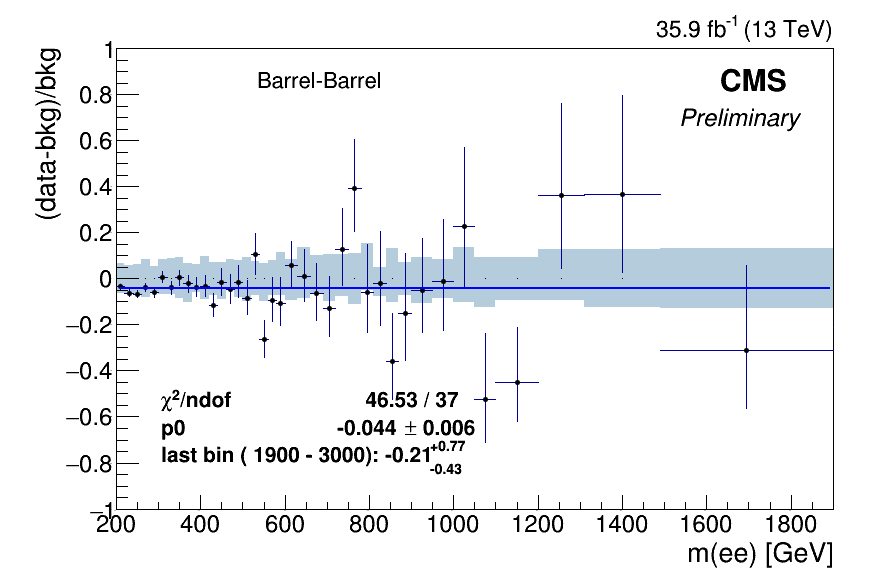
\includegraphics[width=0.47\textwidth]{figures/Zprime/2016/mass/SignalRegionHistEBEB_ratio}
    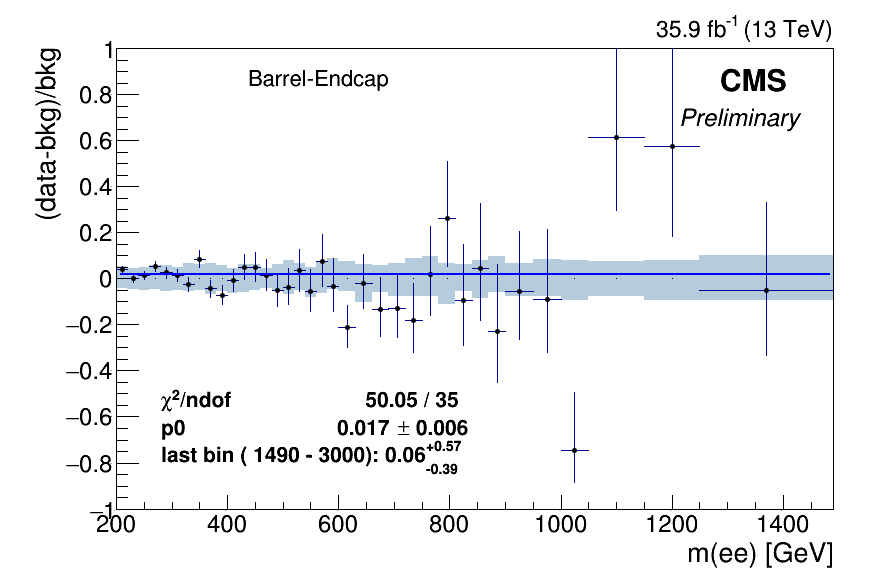
\includegraphics[width=0.47\textwidth]{figures/Zprime/2016/mass/SignalRegionHistEBEE_ratio}
    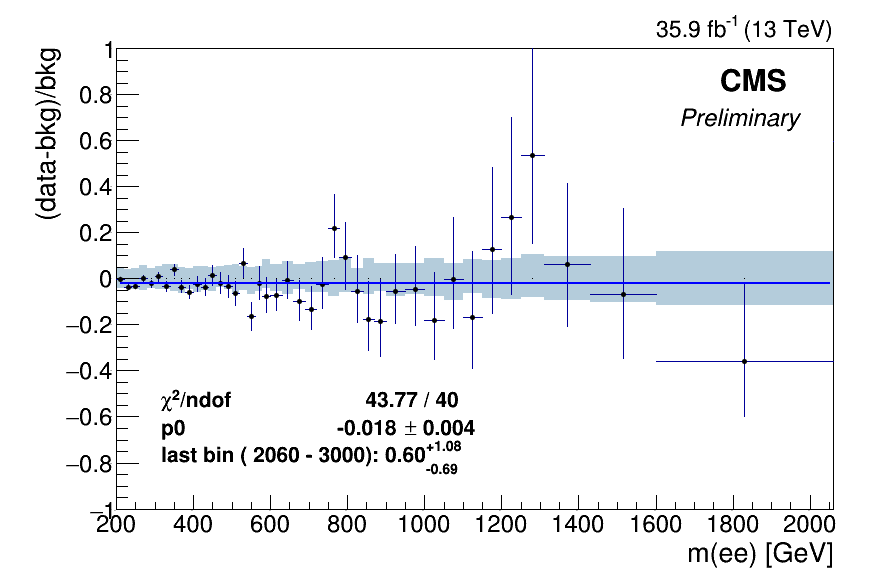
\includegraphics[width=0.47\textwidth]{figures/Zprime/2016/mass/SignalRegionHist_ratio}
    \caption{The ratio of observed dielectron mass spectrum in signal region for barrel-barrel (top left), barrel-endcap (top right) and sum of the barrel-barrel and the barrel-endcap together (bottom) in 2016.}
    \label{massratio_2016}
  \end{center}
\end{figure}

\begin{figure}[!htbp]
  \begin{center}
    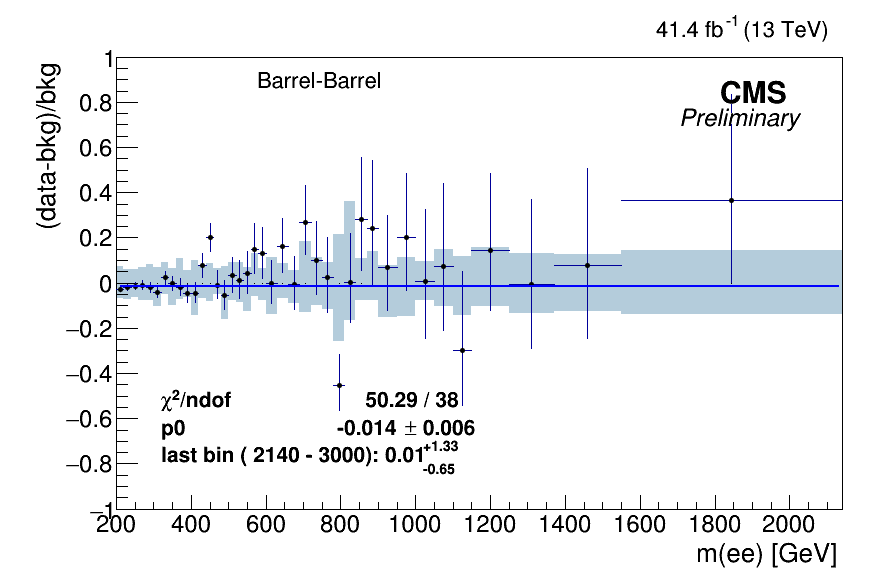
\includegraphics[width=0.47\textwidth]{figures/Zprime/2017/mass/SignalRegionHistEBEB}
    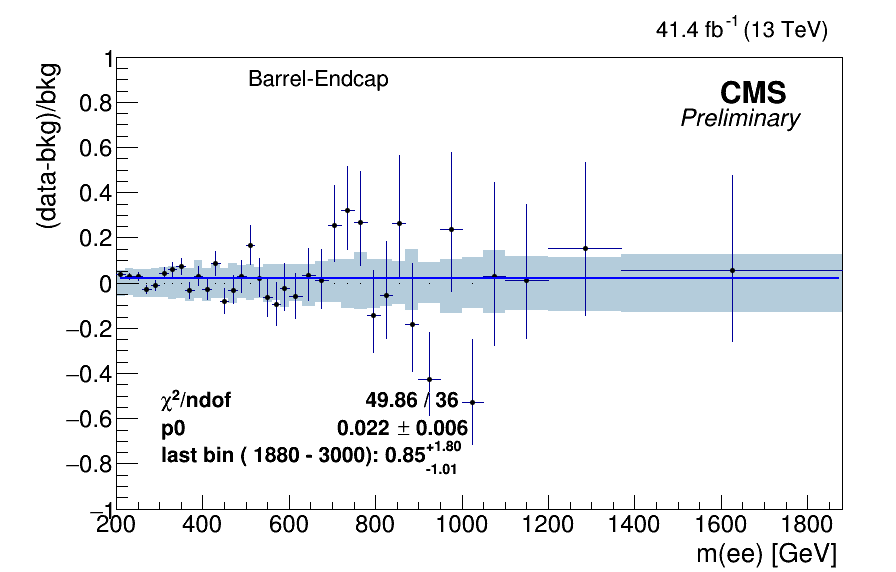
\includegraphics[width=0.47\textwidth]{figures/Zprime/2017/mass/SignalRegionHistEBEE}
    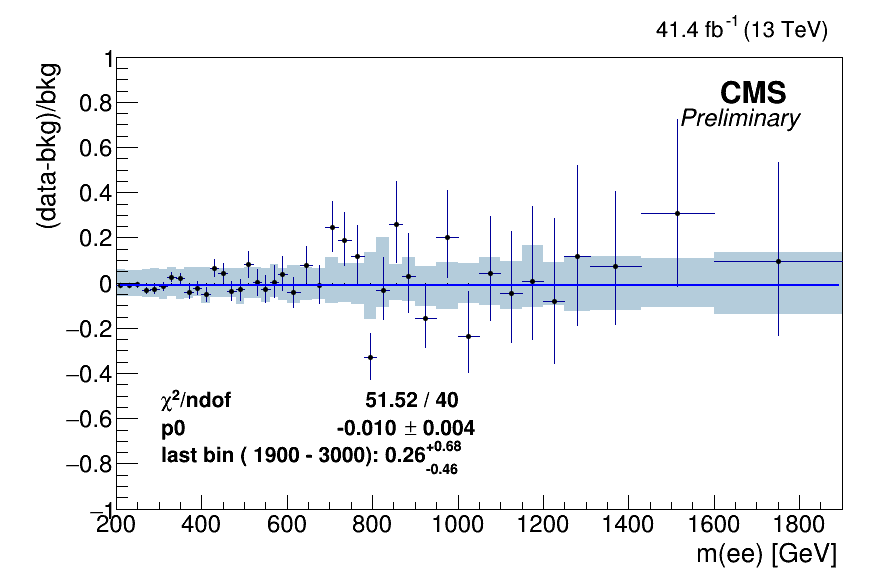
\includegraphics[width=0.47\textwidth]{figures/Zprime/2017/mass/SignalRegionHist}
    \caption{The ratio of observed dielectron mass spectrum in signal region for barrel-barrel (top left), barrel-endcap (top right) and sum of the barrel-barrel and the barrel-endcap together (bottom) in 2017.}
    \label{massratio_2017}
  \end{center}
\end{figure}



In Table \ref{data-MCn}, predicted SM background and observed data yields are shown as a function of dielectron invariant mass.

\begin{table}[!htbp]
\small

\begin{center}
\scalebox{0.8}{
  \begin{tabular}{|l|l|l|l|l|l|l|}
    \hline
Year&Mass range (GeV)   & Data      & Total bkg                 & $\gamma^*$/Z $\rightarrow$ ee    & $\ttbar$ and $\ttbar$-like bkg  & Jets\\ \hline \hline
\multirow{24}{*}{2016}&\multicolumn{6}{c|}{Barrel-Barrel} \\ \cline{2-7}
& 60    -- 120   & 5760346     & 5762889.7  $\pm$ 133911.3 & 5730973.8  $\pm$ 133096.7         & 29369.6    $\pm$ 1277.6    & 2546.3     $\pm$ 1273.2   \\
& 120   -- 400   & 146598      & 152496.1   $\pm$ 11452.7  & 120819.5   $\pm$ 10364.5          & 29824.2    $\pm$ 1572.3    & 1852.5     $\pm$ 926.2    \\
& 400   -- 600   & 2163        & 2295.3     $\pm$ 183.6    & 1636.5     $\pm$ 124.6            & 643.5      $\pm$ 63.2      & 15.4       $\pm$ 7.7      \\
& 600   -- 900   & 523         & 520.1      $\pm$ 51.1     & 425.9      $\pm$ 39.2             & 91.8       $\pm$ 13.3      & 2.4        $\pm$ 1.2      \\
& 900   -- 1300  & 100         & 107.9      $\pm$ 10.6     & 96.5       $\pm$ 9.4              & 10.9       $\pm$ 1.8       & 0.6        $\pm$ 0.3      \\
& 1300  -- 1800  & 24          & 21.5       $\pm$ 2.8      & 20.5       $\pm$ 2.6              & 0.9        $\pm$ 0.2       & 0.1        $\pm$ 0.0      \\
& 1800  -- 6000  & 3           & 5.4        $\pm$ 0.9      & 5.2        $\pm$ 0.9              & 0.2        $\pm$ 0.0       & 0.0        $\pm$ 0.0      \\ \cline{2-7}
&\multicolumn{6}{c|}{Barrel-Endcap} \\ \cline{2-7}
& 60    -- 120   & 2051759     & 2054401.1  $\pm$ 40405.8  & 2042472.6  $\pm$ 40296.8          & 9270.3     $\pm$ 345.6     & 2658.2     $\pm$ 1329.1   \\
& 120   -- 400   & 98503       & 99151.9    $\pm$ 4158.3   & 77350.1    $\pm$ 3306.5           & 17813.2    $\pm$ 728.6     & 3988.6     $\pm$ 1994.3   \\
& 400   -- 600   & 2134        & 2117.0     $\pm$ 112.6    & 1243.8     $\pm$ 58.0             & 751.3      $\pm$ 44.6      & 121.9      $\pm$ 61.0     \\
& 600   -- 900   & 420         & 463.3      $\pm$ 27.9     & 311.7      $\pm$ 18.5             & 128.3      $\pm$ 9.9       & 23.2       $\pm$ 11.6     \\
& 900   -- 1300  & 82          & 78.4       $\pm$ 5.9      & 59.2       $\pm$ 4.6              & 15.9       $\pm$ 1.6       & 3.3        $\pm$ 1.7      \\
& 1300  -- 1800  & 9           & 12.8       $\pm$ 1.2      & 10.3       $\pm$ 1.0              & 1.9        $\pm$ 0.4       & 0.6        $\pm$ 0.3      \\
& 1800  -- 6000  & 6           & 2.1        $\pm$ 0.3      & 1.8        $\pm$ 0.2              & 0.1        $\pm$ 0.0       & 0.1        $\pm$ 0.1      \\ \cline{2-7}
&\multicolumn{6}{c|}{Barrel-Barrel + Barrel-Endcap} \\ \cline{2-7}
& 60    -- 120   & 7812105     & 7817300.8  $\pm$ 166656.9 & 7773476.7  $\pm$ 165766.3         & 38627.6    $\pm$ 1524.1    & 5196.5     $\pm$ 2598.2   \\
& 120   -- 400   & 245101      & 252071.4   $\pm$ 12933.9  & 198526.1   $\pm$ 11326.7          & 47709.5    $\pm$ 2148.8    & 5835.8     $\pm$ 2917.9   \\
& 400   -- 600   & 4297        & 4424.5     $\pm$ 232.4    & 2887.1     $\pm$ 147.9            & 1400.2     $\pm$ 87.6      & 137.2      $\pm$ 68.6     \\
& 600   -- 900   & 943         & 985.9      $\pm$ 63.9     & 739.3      $\pm$ 48.7             & 221.0      $\pm$ 17.2      & 25.6       $\pm$ 12.8     \\
& 900   -- 1300  & 182         & 186.6      $\pm$ 13.5     & 155.9      $\pm$ 11.9             & 26.8       $\pm$ 2.3       & 3.9        $\pm$ 1.9      \\
& 1300  -- 1800  & 33          & 34.3       $\pm$ 3.4      & 30.9       $\pm$ 3.2              & 2.8        $\pm$ 0.5       & 0.6        $\pm$ 0.3      \\
& 1800  -- 6000  & 9           & 7.5        $\pm$ 1.1      & 7.0        $\pm$ 1.1              & 0.3        $\pm$ 0.0       & 0.1        $\pm$ 0.1      \\  \cline{2-7} \hline \hline
\multirow{24}{*}{2017}& \multicolumn{6}{c|}{Barrel-Barrel} \\ \cline{2-7}
& 60    -- 120   & 6190697        & 6194808.2  $\pm$ 178177.2   & 6156571.2  $\pm$ 177324.0         & 34116.3    $\pm$ 1921.1           & 4120.7      \\
& 120   -- 400   & 162005         & 167925.2   $\pm$ 13932.9    & 132981.8   $\pm$ 12618.8          & 33128.5    $\pm$ 2365.8           & 1815.0      \\
& 400   -- 600   & 2503           & 2404.7     $\pm$ 215.9      & 1782.7     $\pm$ 144.5            & 605.2      $\pm$ 79.6             & 16.8        \\
& 600   -- 900   & 588            & 560.2      $\pm$ 51.5       & 478.6      $\pm$ 44.9             & 78.7       $\pm$ 15.6             & 3.0         \\
& 900   -- 1300  & 118            & 113.4      $\pm$ 13.1       & 105.1      $\pm$ 11.4             & 7.8        $\pm$ 2.8              & 0.5         \\
& 1300  -- 1800  & 28             & 23.1       $\pm$ 3.0        & 23.0       $\pm$ 3.0              & 0.0        $\pm$ 0.0              & 0.1         \\
& 1800  -- 6000  & 7              & 5.7        $\pm$ 1.0        & 5.7        $\pm$ 1.0              & 0.0        $\pm$ 0.0              & 0.0         \\  \cline{2-7}
&\multicolumn{6}{c|}{Barrel-Endcap} \\ \cline{2-7}
& 60    -- 120   & 2096490        & 2098260.5  $\pm$ 96902.6    & 2086010.3  $\pm$ 96566.8          & 10473.3    $\pm$ 675.3            & 1777.0     \\
& 120   -- 400   & 109771         & 110357.8   $\pm$ 6227.6     & 87277.3    $\pm$ 5107.0           & 19860.0    $\pm$ 1450.6           & 3220.6     \\
& 400   -- 600   & 2365           & 2364.5     $\pm$ 164.6      & 1442.8     $\pm$ 99.9             & 810.5      $\pm$ 68.3             & 111.3      \\
& 600   -- 900   & 518            & 488.3      $\pm$ 37.9       & 341.8      $\pm$ 26.5             & 124.1      $\pm$ 13.9             & 22.4       \\
& 900   -- 1300  & 75             & 86.5       $\pm$ 7.7        & 69.5       $\pm$ 6.3              & 14.0       $\pm$ 2.7              & 3.0        \\
& 1300  -- 1800  & 16             & 14.2       $\pm$ 1.7        & 11.7       $\pm$ 1.3              & 2.0        $\pm$ 1.0              & 0.6        \\
& 1800  -- 6000  & 3              & 2.2        $\pm$ 0.3        & 2.1        $\pm$ 0.3              & 0.0        $\pm$ 0.0              & 0.1        \\  \cline{2-7}
&\multicolumn{6}{c|}{Barrel-Barrel + Barrel-Endcap} \\ \cline{2-7}
& 60    -- 120   & 8287187        & 8290233.1  $\pm$ 369104.3   & 8242650.8  $\pm$ 364680.2         & 44535.5    $\pm$ 2834.7           & 3046.7    \\
& 120   -- 400   & 271776         & 280802.3   $\pm$ 18298.7    & 222376.6   $\pm$ 15710.7          & 53411.9    $\pm$ 3976.3           & 5013.9    \\
& 400   -- 600   & 4868           & 4841.2     $\pm$ 329.4      & 3267.6     $\pm$ 216.8            & 1446.0     $\pm$ 128.0            & 127.6     \\
& 600   -- 900   & 1106           & 1062.0     $\pm$ 77.4       & 829.4      $\pm$ 63.0             & 207.4      $\pm$ 22.6             & 25.3      \\
& 900   -- 1300  & 193            & 201.3      $\pm$ 18.0       & 176.2      $\pm$ 16.0             & 21.6       $\pm$ 3.9              & 3.5       \\
& 1300  -- 1800  & 44             & 37.6       $\pm$ 4.2        & 34.8       $\pm$ 4.0              & 2.1        $\pm$ 1.1              & 0.7       \\
& 1800  -- 6000  & 10             & 7.9        $\pm$ 1.2        & 7.8        $\pm$ 1.2              & 0.0        $\pm$ 0.0              & 0.1       \\  \hline

\end{tabular}}
\end{center}
\caption{Predicted SM background and observed data yields as a function of dielectron invariant mass for Barrel-Barrel, Barrel-Endcap and Barrel-Barrel plus Barrel-Endcap regions. The uncertainty contains statistic uncertainty and systematic uncertainty.}
\label{data-MCn}
\end{table}




In Table \ref{systematic_effect}, the relative effect of each systematic uncertainty is shown as a function of dielectron invariant mass.

\begin{table}[!htbp]
\small

\begin{center}
\scalebox{0.8}{
\begin{tabular}{|l|l|l|l|l|l|l|l|l|}
\hline
Year&Uncertainty             & 60-120 GeV     & 120-400 GeV    & 400-600 GeV    & 600-900 GeV   & 900-1300 GeV   & 1300-1800 GeV  & 1800-6000 GeV \\\hline
\multirow{14}{*}{2016}&Normalization\_scale\_up    & 0.998\%        & 0.972\%        & 0.966\%        &0.971\%        & 0.977\%        & 0.980\%        & 0.982\%    \\\cline{2-9}
&Normalization\_scale\_down  & 0.998\%        & 0.972\%        & 0.966\%        &0.971\%        & 0.977\%        & 0.980\%        & 0.982\%    \\\cline{2-9}
&Pdf\_scale\_up              & 0.147\%        & 0.165\%        & 1.122\%        &2.215\%        & 3.753\%        & 6.279\%        & 10.351\%   \\\cline{2-9}
&Pdf\_scale\_down            & 0.096\%        & 0.025\%        & 1.000\%        &1.774\%        & 3.769\%        & 6.397\%        & 9.928\%    \\\cline{2-9}
&Energy\_scale\_up           & 0.201\%        & 4.473\%        & 4.147\%        &4.925\%        & 4.830\%        & 6.523\%        & 8.699\%    \\\cline{2-9}
&Energy\_scale\_down         & 0.095\%        & 4.325\%        & 3.930\%        &3.942\%        & 5.073\%        & 5.614\%        & 6.873\%    \\\cline{2-9}
&PU\_scale\_up               & 0.472\%        & 0.446\%        & 0.405\%        &0.827\%        & 0.323\%        & 0.050\%        & 0.729\%    \\\cline{2-9}
&PU\_scale\_down             & 0.424\%        & 0.262\%        & 0.353\%        &0.264\%        & 0.394\%        & 0.367\%        & 0.349\%    \\\cline{2-9}
&Bgk\_scale\_up              & 0.036\%        & 1.334\%        & 1.870\%        &1.460\%        & 1.092\%        & 0.958\%        & 0.888\%    \\\cline{2-9}
&Bgk\_scale\_down            & 0.036\%        & 1.334\%        & 1.870\%        &1.460\%        & 1.092\%        & 0.958\%        & 0.888\%    \\\cline{2-9}
&SF\_scale\_up               & 1.797\%        & 1.778\%        & 2.078\%        &2.893\%        & 3.065\%        & 3.590\%        & 4.949\%    \\\cline{2-9}
&SF\_scale\_down             & 1.711\%        & 1.510\%        & 1.991\%        &2.144\%        & 3.072\%        & 3.836\%        & 4.355\%    \\\cline{2-9}
&Total\_scale\_up            & 2.124\%        & 5.111\%        & 5.231\%        &6.426\%        & 7.004\%        & 9.836\%        & 14.477\%   \\\cline{2-9}
&Total\_scale\_down          & 2.031\%        & 4.877\%        & 4.996\%        &5.141\%        & 7.188\%        & 9.443\%        & 12.909\%   \\\hline \hline
\multirow{14}{*}{2017}&Normalization\_scale\_up    & 4.033\%        & 3.900\%        & 3.882\%        & 3.895\%        & 3.922\%        & 3.922\%        & 3.937\%        \\\cline{2-9}
&Normalization\_scale\_down  & 3.992\%        & 3.900\%        & 3.882\%        & 3.895\%        & 3.922\%        & 3.922\%        & 3.937\%        \\\cline{2-9}
&Pdf\_scale\_up              & 0.114\%        & 0.125\%        & 1.021\%        & 2.102\%        & 3.941\%        & 6.456\%        & 10.549\%       \\\cline{2-9}
&Pdf\_scale\_down            & 0.114\%        & 0.125\%        & 1.021\%        & 2.102\%        & 3.941\%        & 6.456\%        & 10.549\%       \\\cline{2-9}
&Energy\_scale\_up           & 0.217\%        & 4.312\%        & 4.009\%        & 4.562\%        & 4.382\%        & 5.875\%        & 8.415\%        \\\cline{2-9}
&Energy\_scale\_down         & 0.143\%        & 4.660\%        & 4.312\%        & 4.144\%        & 5.083\%        & 5.335\%        & 7.396\%        \\\cline{2-9}
&PU\_scale\_up               & 0.446\%        & 0.315\%        & 0.215\%        & 0.510\%        & 0.344\%        & 0.000\%        & 0.414\%        \\\cline{2-9}
&PU\_scale\_down             & 0.480\%        & 0.338\%        & 0.247\%        & 0.427\%        & 0.283\%        & 0.096\%        & 0.422\%        \\\cline{2-9}
&Bkg\_scale\_up              & 0.029\%        & 1.391\%        & 2.036\%        & 1.491\%        & 0.959\%        & 0.952\%        & 0.773\%        \\\cline{2-9}
&Bkg\_scale\_down            & 0.029\%        & 1.391\%        & 2.036\%        & 1.491\%        & 0.959\%        & 0.952\%        & 0.773\%        \\\cline{2-9}
&SF\_scale\_up               & 1.805\%        & 1.515\%        & 1.670\%        & 2.327\%        & 3.477\%        & 4.648\%        & 5.198\%        \\\cline{2-9}
&SF\_scale\_down             & 1.806\%        & 1.798\%        & 2.627\%        & 3.422\%        & 4.391\%        & 4.872\%        & 5.162\%        \\\cline{2-9}
&Total\_scale\_up            & 4.448\%        & 6.176\%        & 6.258\%        & 6.950\%        & 7.953\%        & 10.681\%        & 15.012\%      \\\cline{2-9}
&Total\_scale\_down          & 4.412\%        & 6.498\%        & 6.768\%        & 7.133\%        & 8.776\%        & 10.496\%        & 14.453\%      \\\hline

\end{tabular}}
\end{center}
\caption{The relative effect of each systematic uncertainty as a function of dielectron invariant mass.}
\label{systematic_effect}
\end{table}



\clearpage
\subsection{Complementary plot}
In addition to the invariant mass plots, the distributions of the following variables are shown in Figure \ref{fig:complementary_2016} (\ref{fig:complementary_2017}) for 2016 (2017).
\begin{itemize}
  \item invariant mass of the selected electron pair in Z peak region for different catagories
  \item \et, $\eta$ and $\phi$ of leading electron and sub-leading electron for $\mathrm{M_{ee}}>200$ GeV
  \item $\Delta R$ and $\Delta\phi$ between selected electrons for $\mathrm{M_{ee}}>200$ GeV
  \item \pt of the reconstructed Z for $\mathrm{M_{ee}}>200$ GeV
\end{itemize}



\begin{figure}[ht]
  \begin{center}
    \begin{tabular}{ccc}
      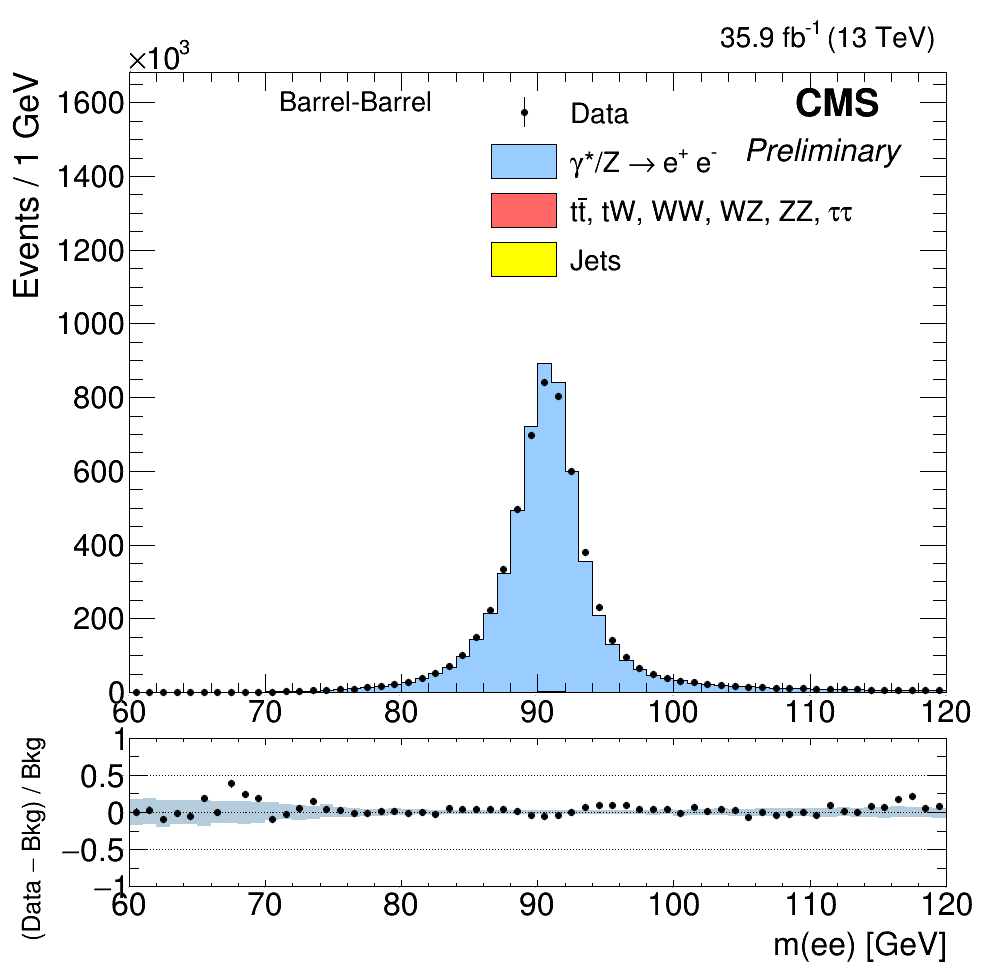
\includegraphics[width=0.32\textwidth]{figures/Zprime/2016/complementary/h_mee_Zpeak_BB.png}&
      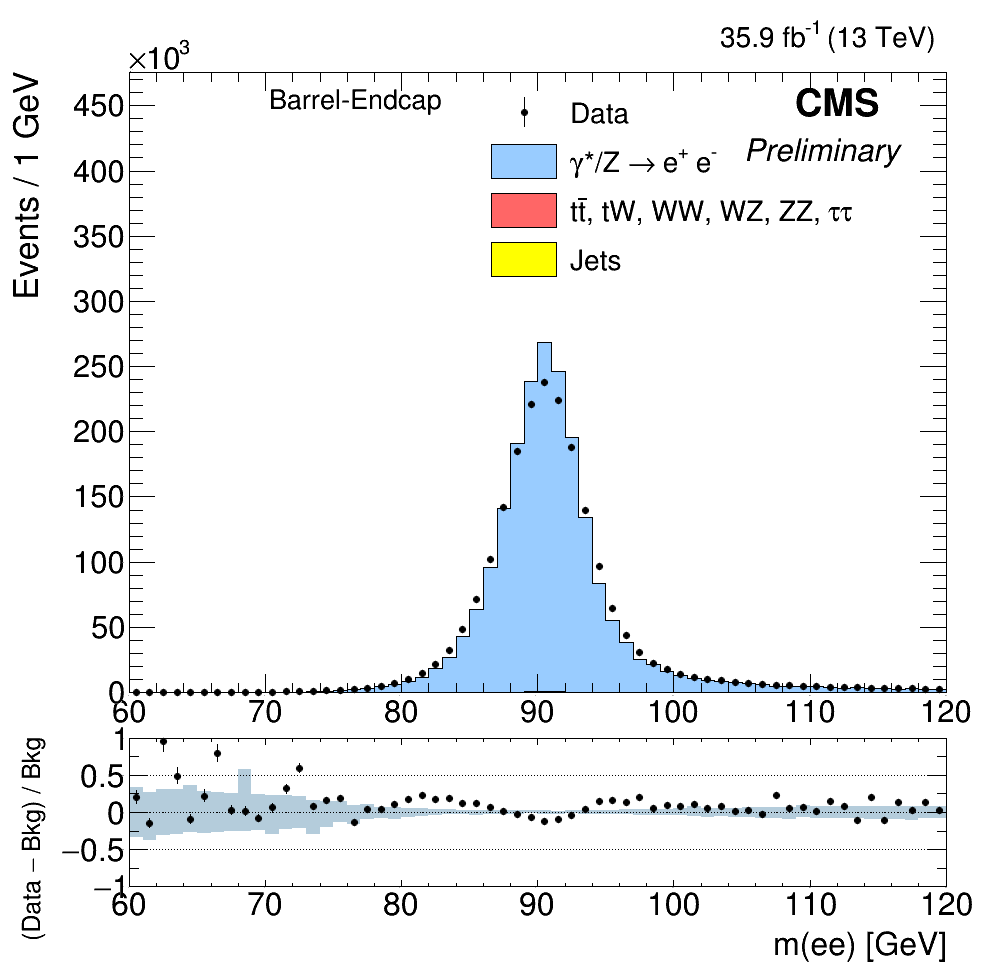
\includegraphics[width=0.32\textwidth]{figures/Zprime/2016/complementary/h_mee_Zpeak_BE.png}&
      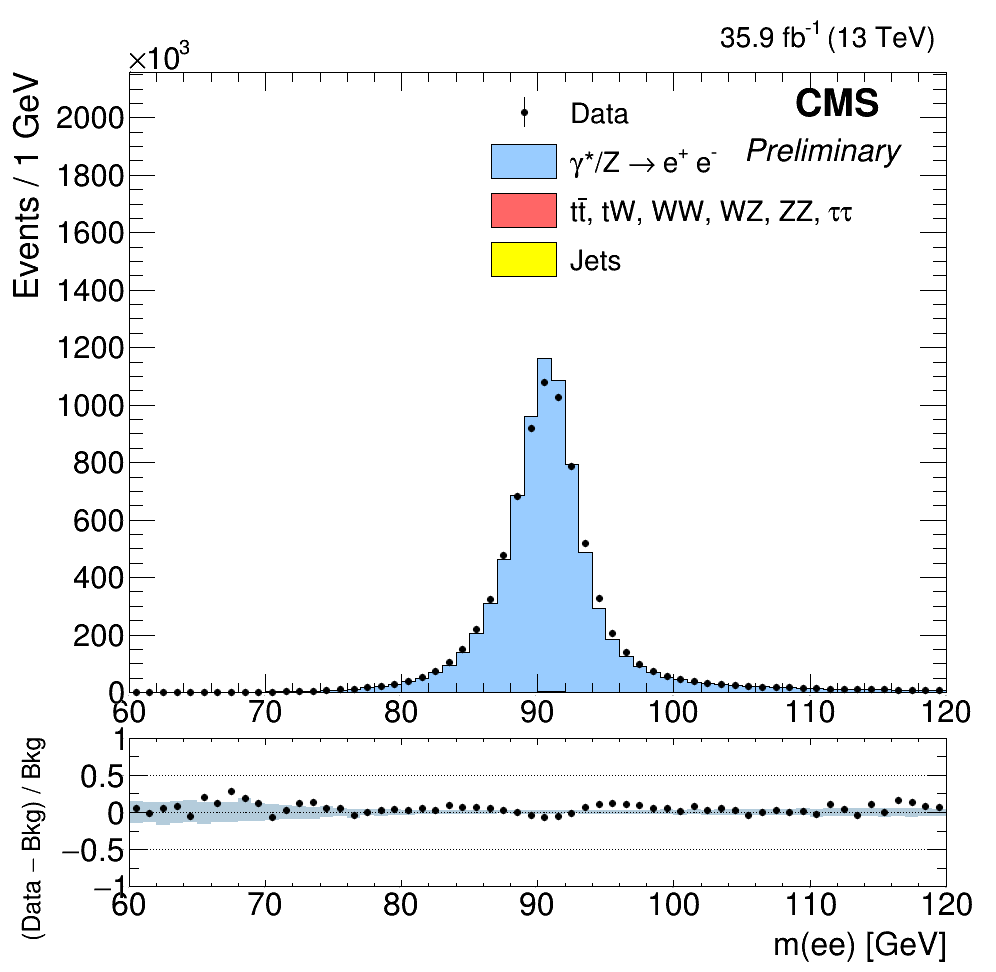
\includegraphics[width=0.32\textwidth]{figures/Zprime/2016/complementary/h_mee_Zpeak.png}\\
      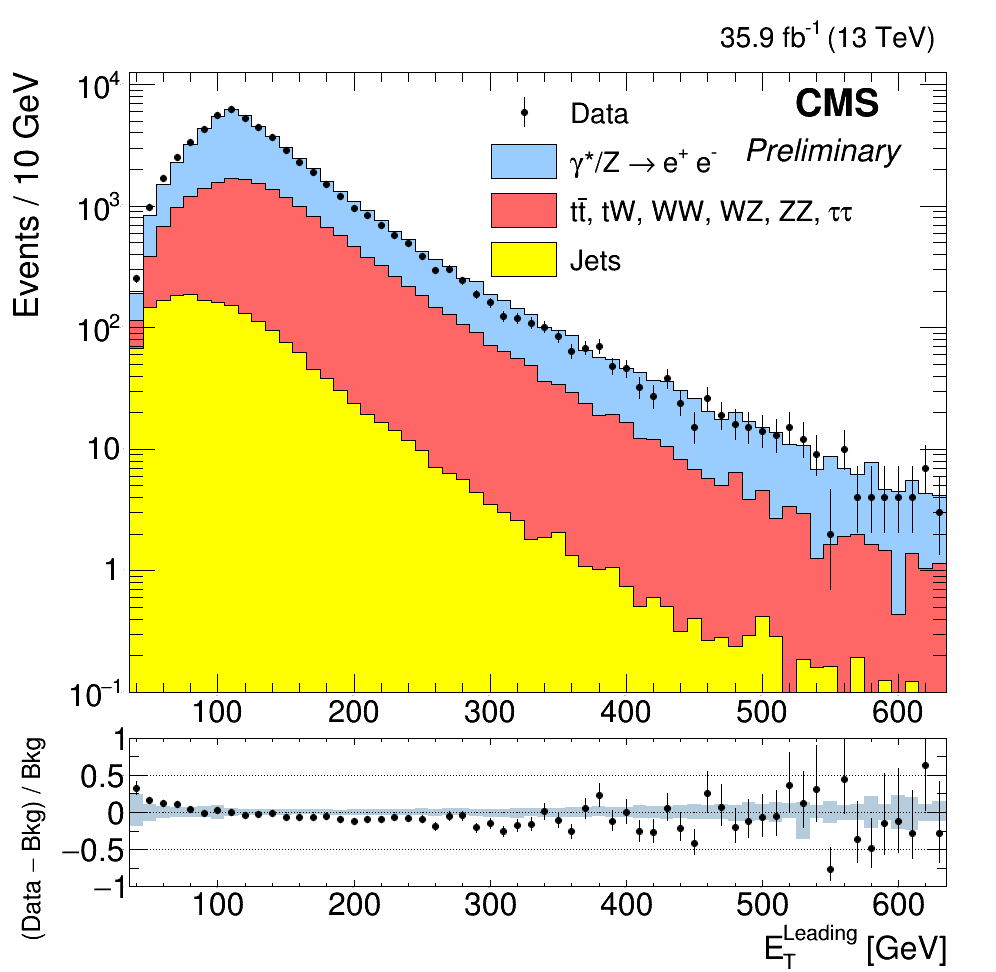
\includegraphics[width=0.32\textwidth]{figures/Zprime/2016/complementary/h_led_Et.png}&
      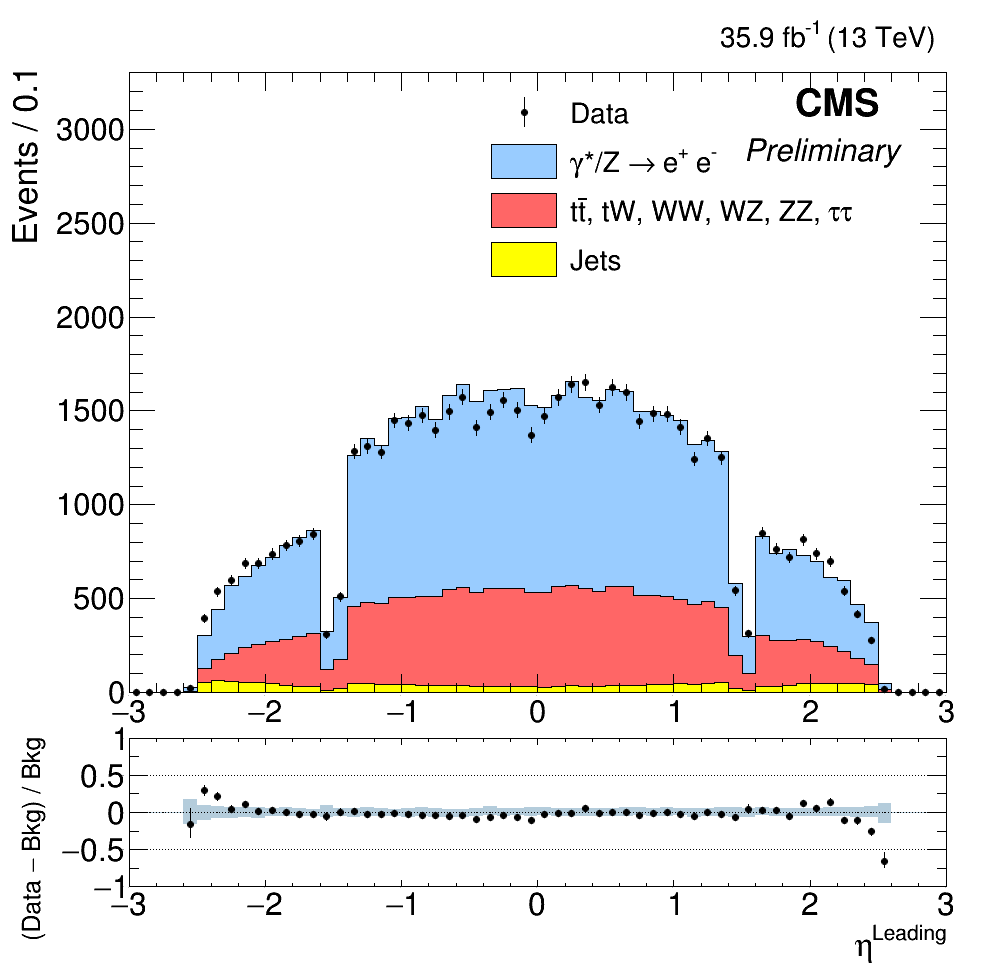
\includegraphics[width=0.32\textwidth]{figures/Zprime/2016/complementary/h_led_eta.png}&
      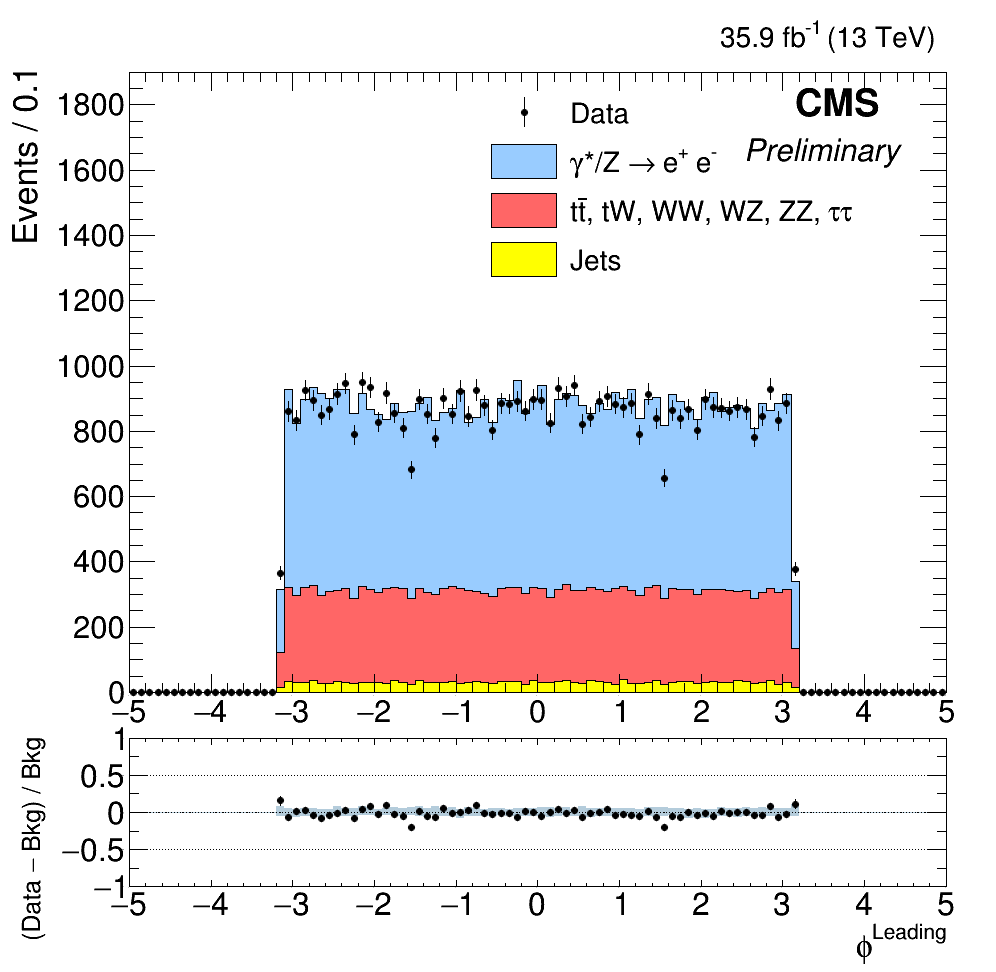
\includegraphics[width=0.32\textwidth]{figures/Zprime/2016/complementary/h_led_phi.png}\\
      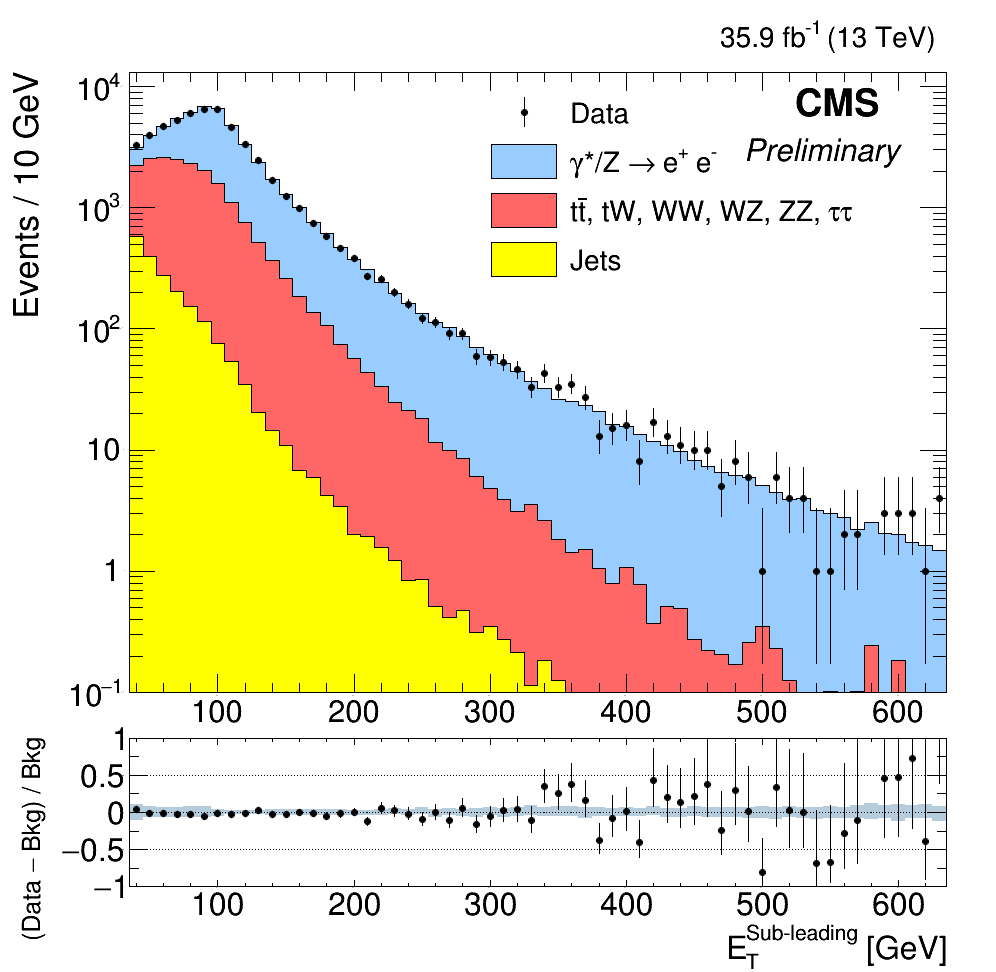
\includegraphics[width=0.32\textwidth]{figures/Zprime/2016/complementary/h_sub_Et.png}&
      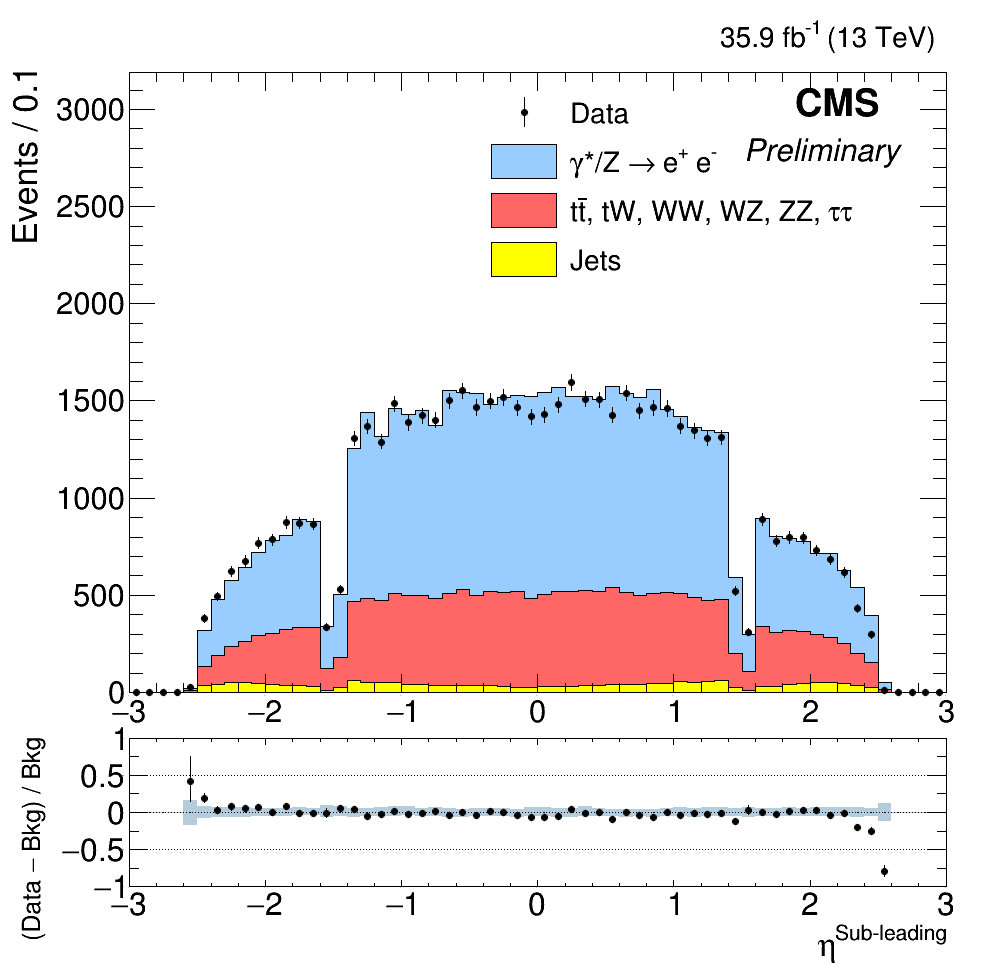
\includegraphics[width=0.32\textwidth]{figures/Zprime/2016/complementary/h_sub_eta.png}&
      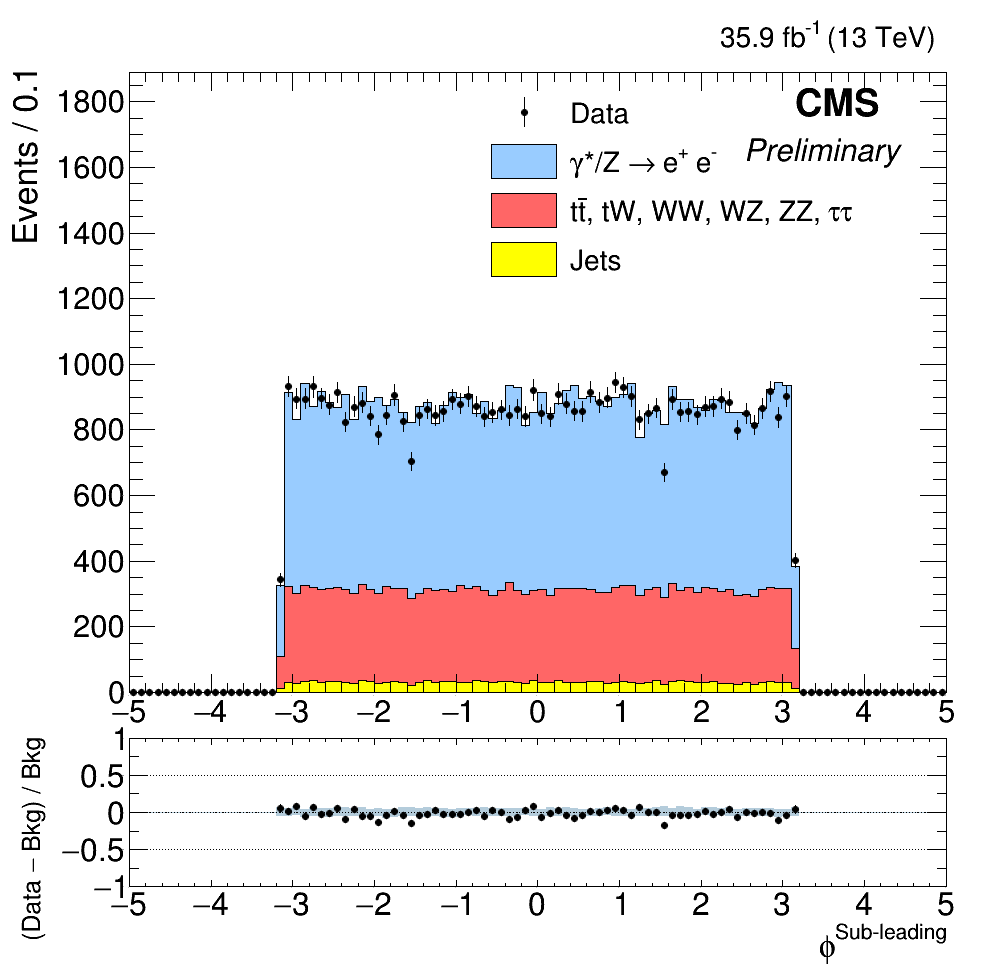
\includegraphics[width=0.32\textwidth]{figures/Zprime/2016/complementary/h_sub_phi.png}\\
      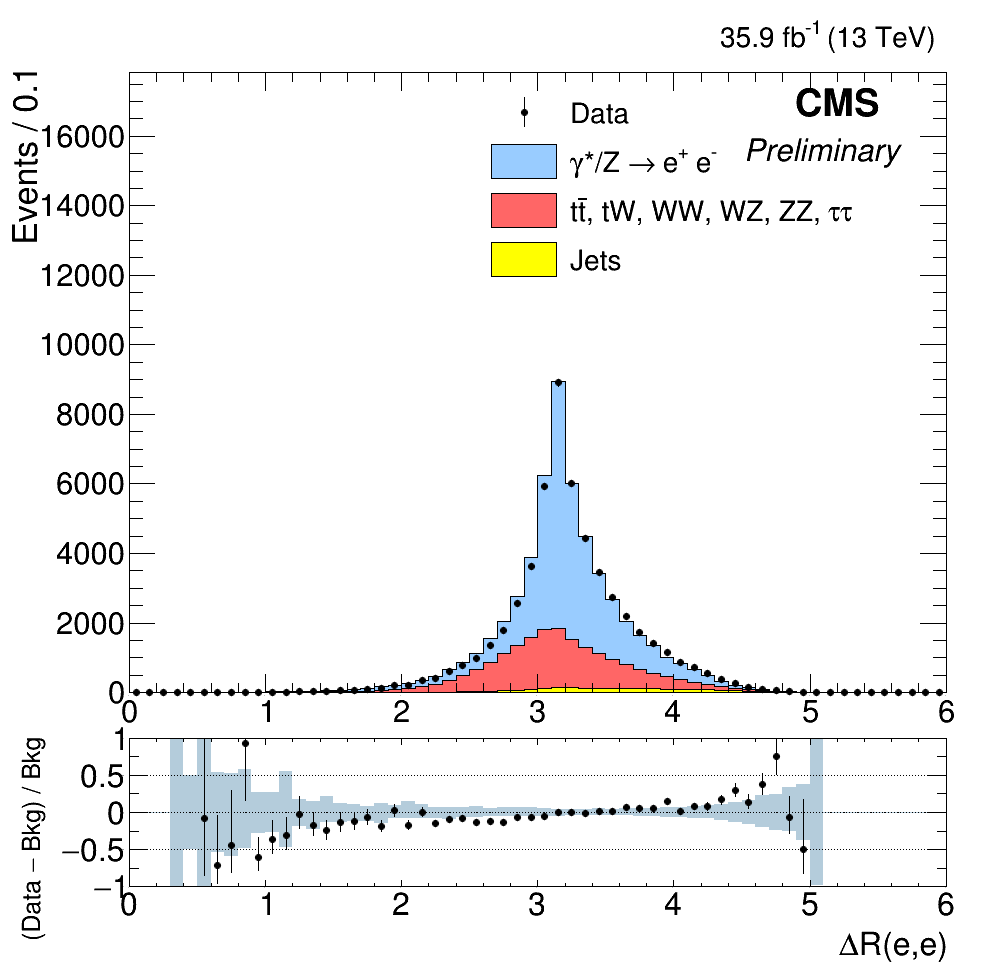
\includegraphics[width=0.32\textwidth]{figures/Zprime/2016/complementary/h_DR_ll.png}&
      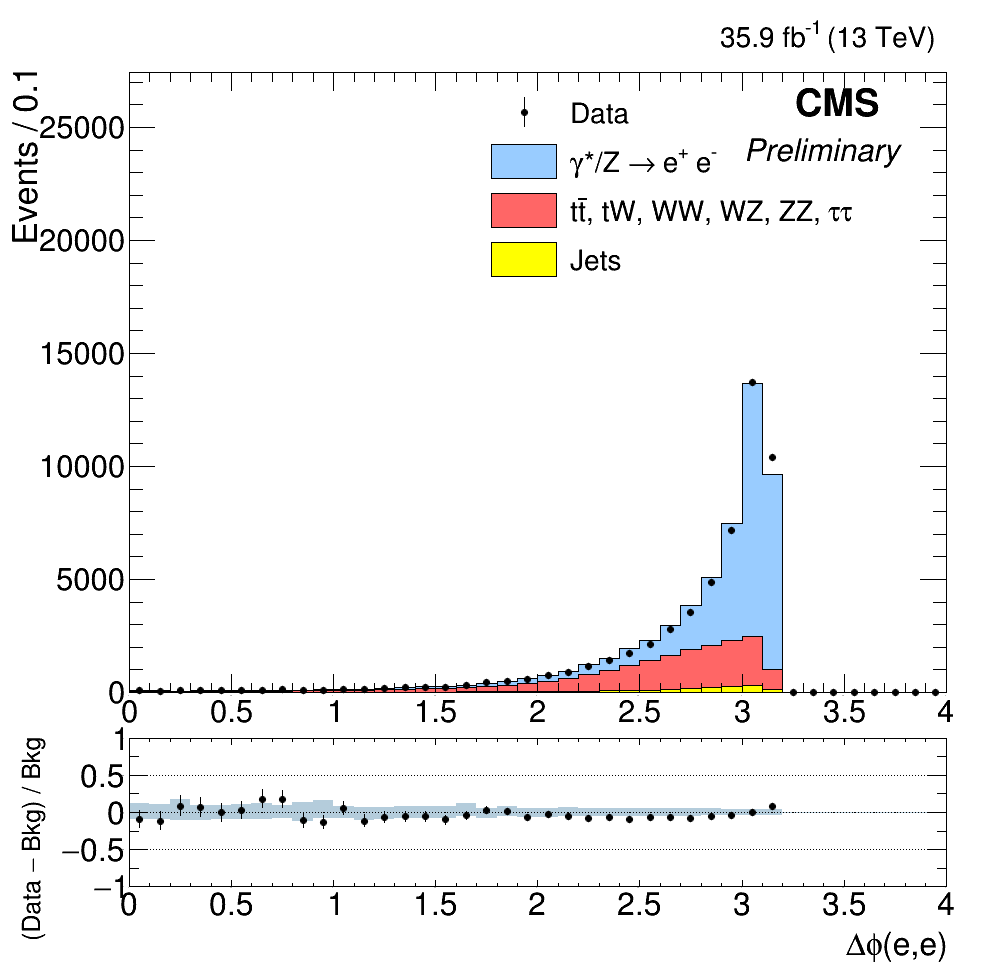
\includegraphics[width=0.32\textwidth]{figures/Zprime/2016/complementary/h_Dphi_ll.png}&
      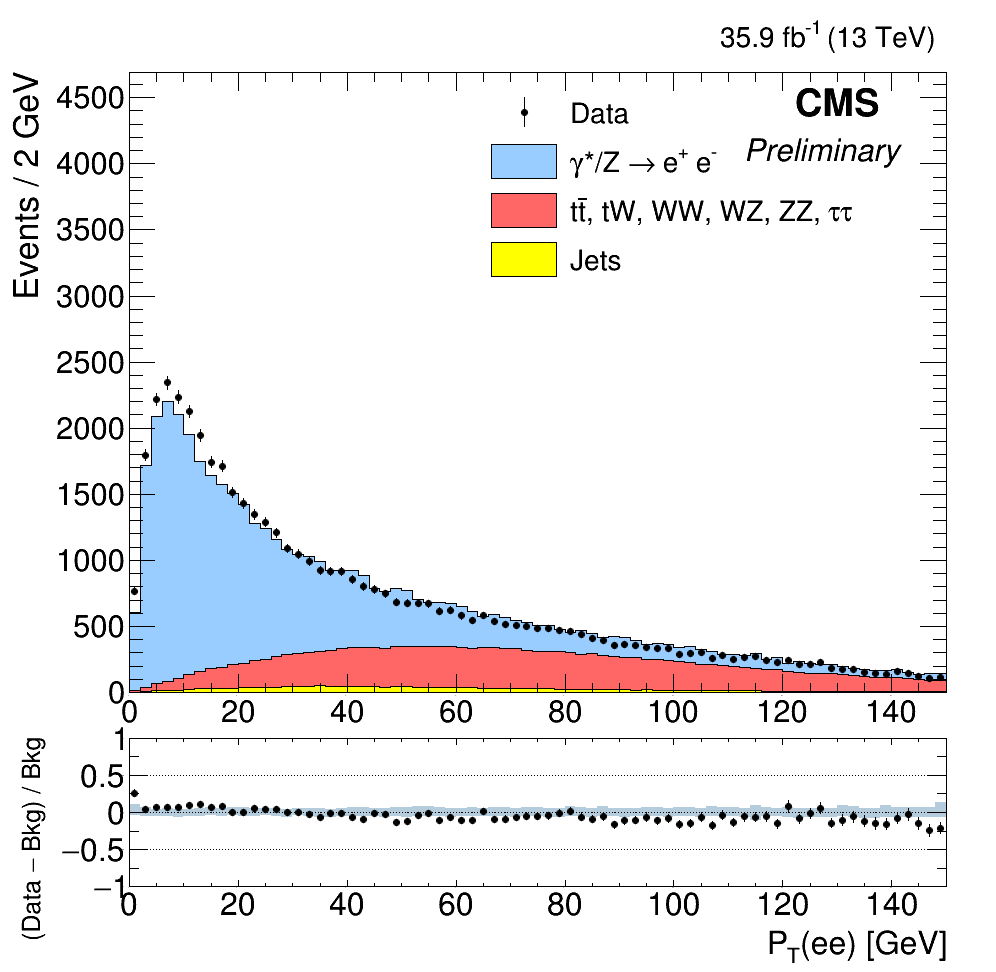
\includegraphics[width=0.32\textwidth]{figures/Zprime/2016/complementary/h_Ptll.png}\\
    \end{tabular}
    \caption{The distributions of invariant mass of two electrons in barrel-barrel, barrel-endcap and barrel-barrel + barrel-endcap (first row), \et, $\eta$ and $\phi$ of leading electron (second row) and \et, $\eta$ and $\phi$ of sub-leading electron (third row),$\Delta R$, $\Delta\phi$ between two electrons and \pt of Z (fourth row) in 2016.
    \label{fig:complementary_2016}}
  \end{center}
\end{figure}

\begin{figure}[ht]
  \begin{center}
    \begin{tabular}{ccc}
      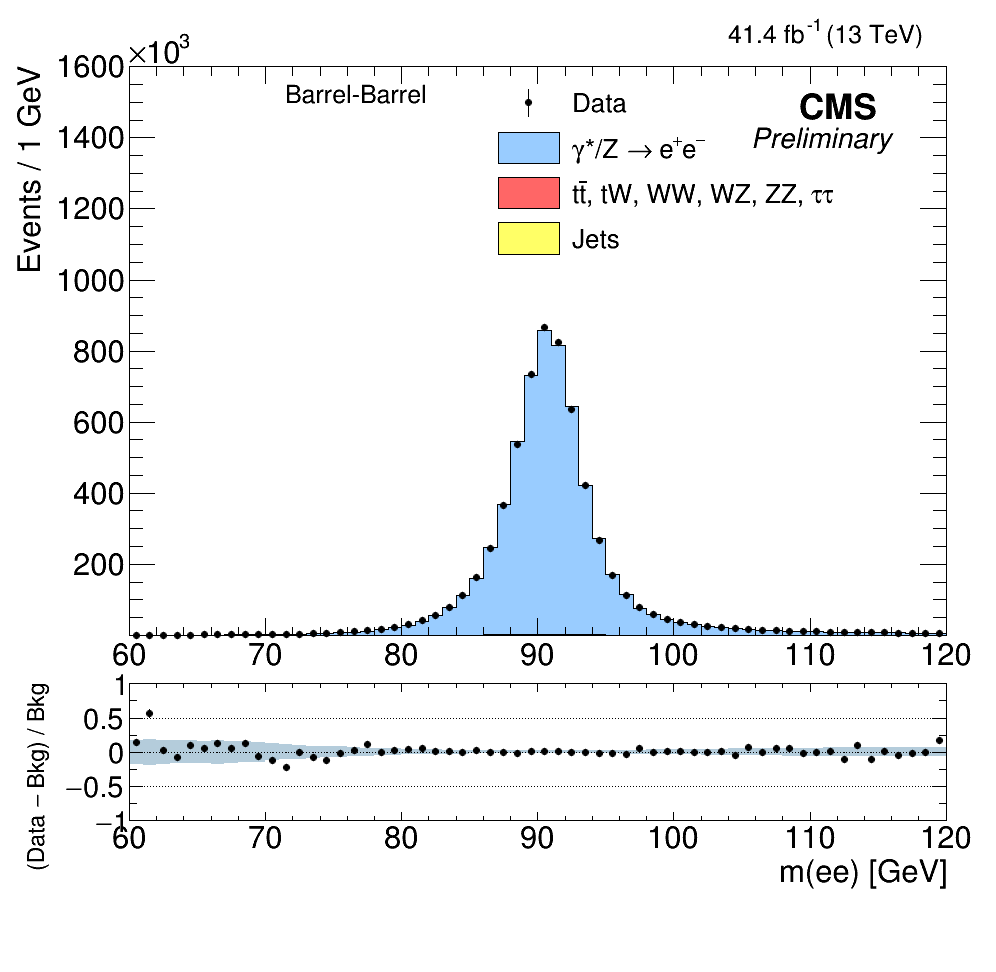
\includegraphics[width=0.32\textwidth]{figures/Zprime/2017/complementary/h_mee_Zpeak_BB.png}&
      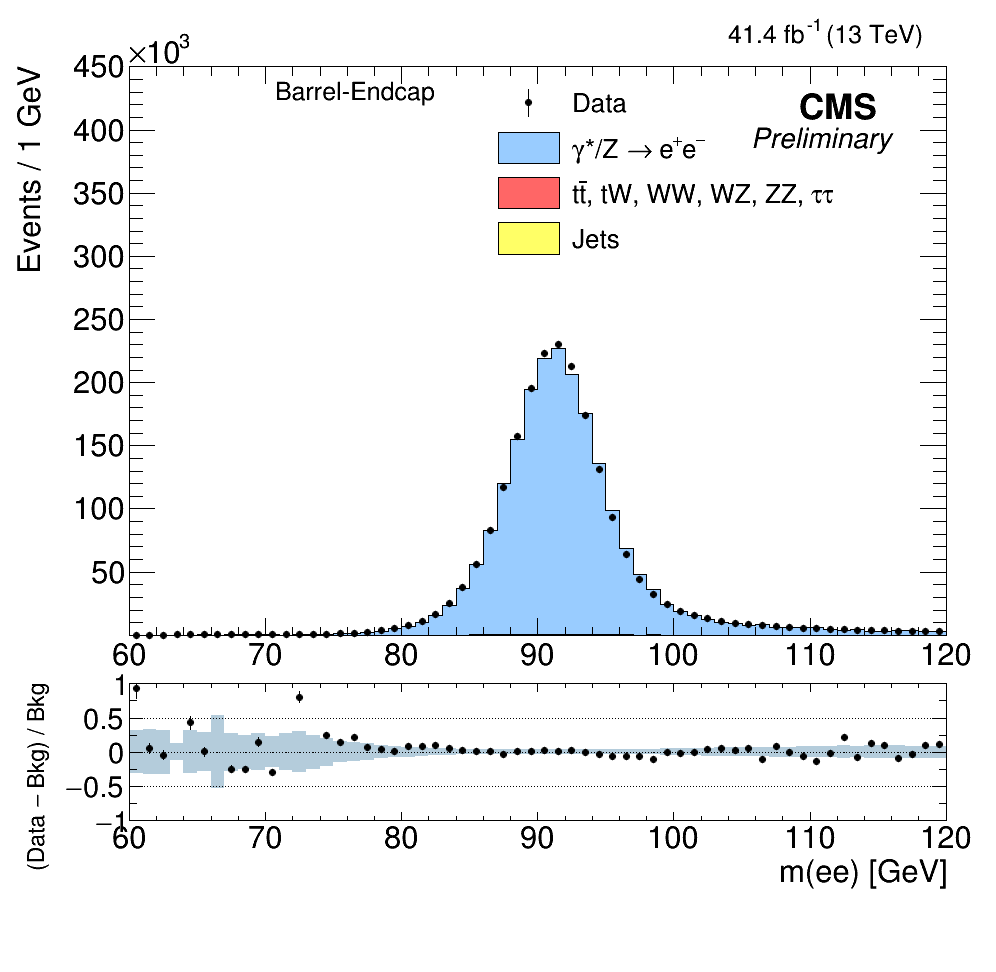
\includegraphics[width=0.32\textwidth]{figures/Zprime/2017/complementary/h_mee_Zpeak_BE.png}&
      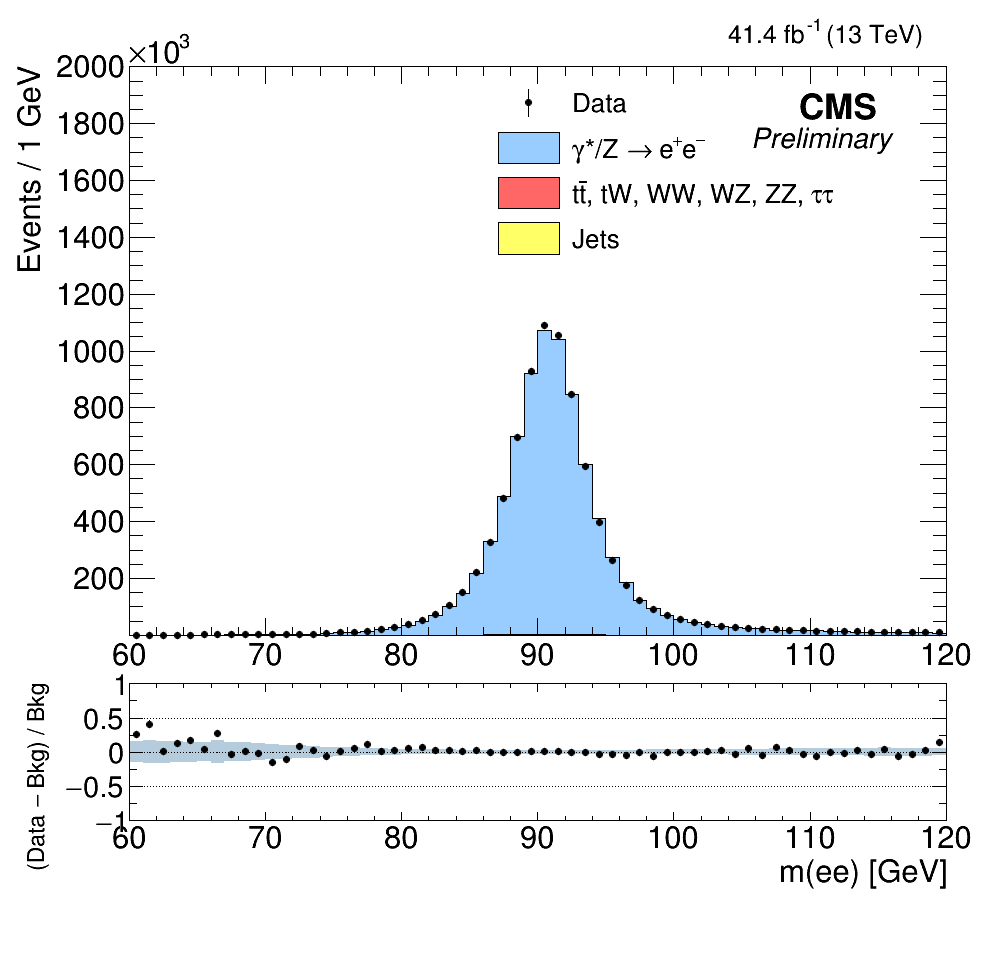
\includegraphics[width=0.32\textwidth]{figures/Zprime/2017/complementary/h_mee_Zpeak.png}\\
      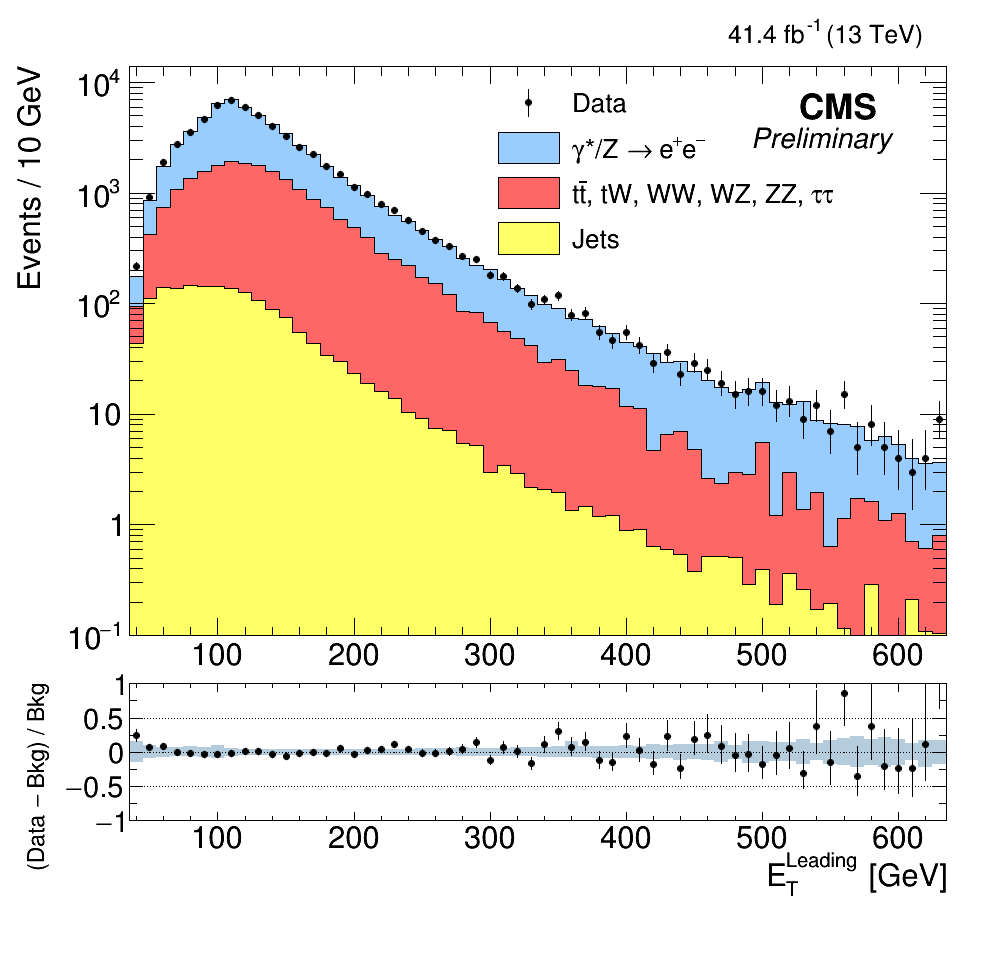
\includegraphics[width=0.32\textwidth]{figures/Zprime/2017/complementary/h_led_Et.png}&
      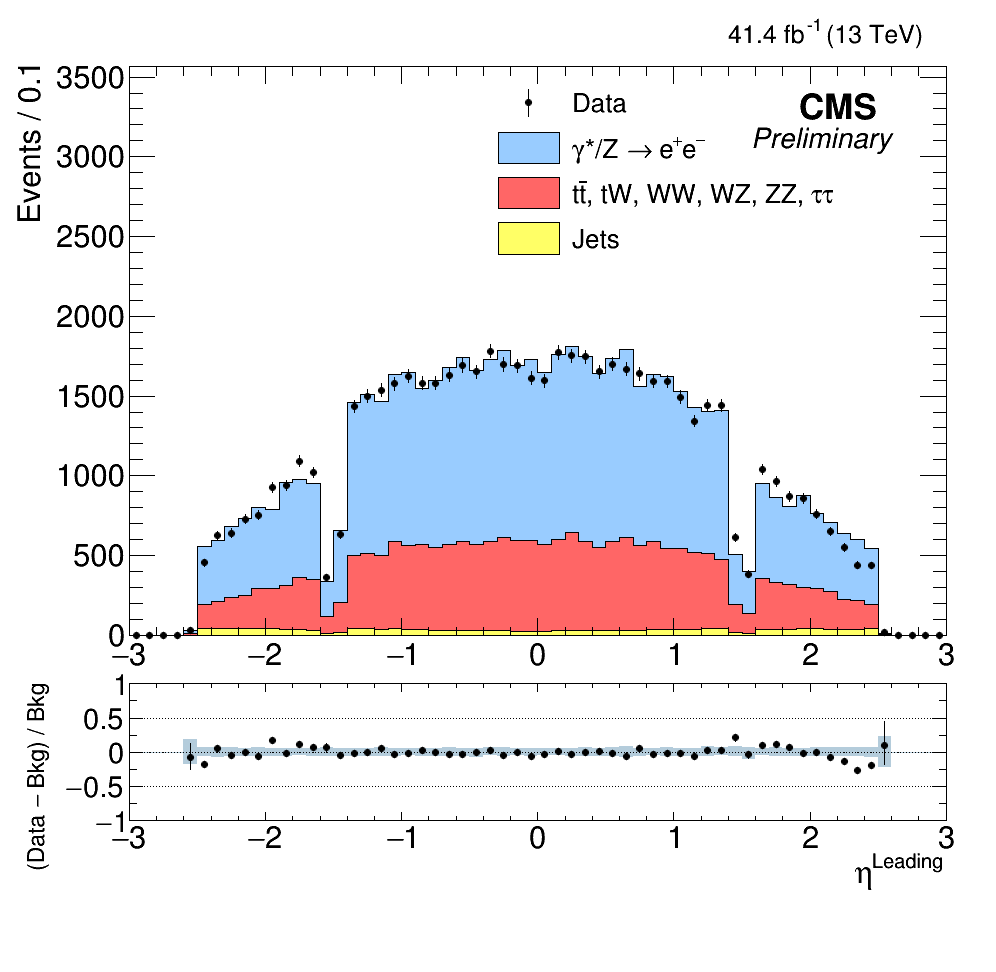
\includegraphics[width=0.32\textwidth]{figures/Zprime/2017/complementary/h_led_eta.png}&
      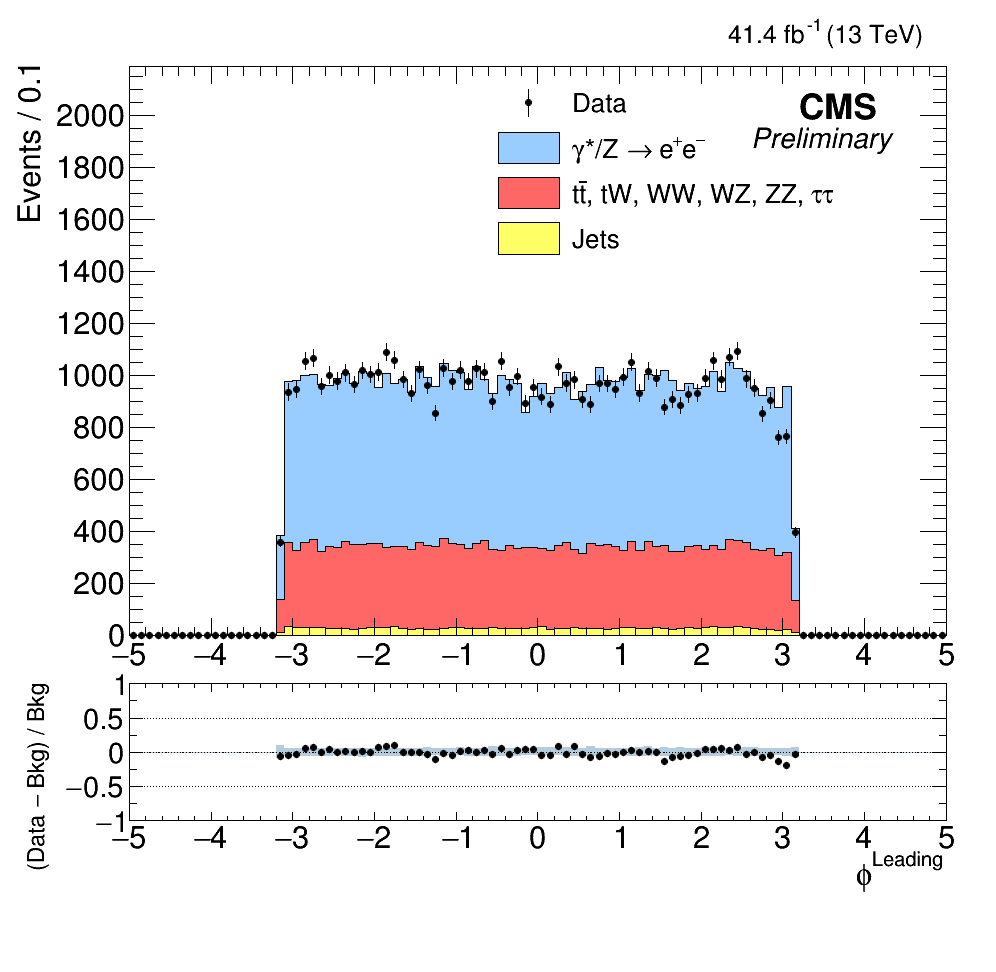
\includegraphics[width=0.32\textwidth]{figures/Zprime/2017/complementary/h_led_phi.png}\\
      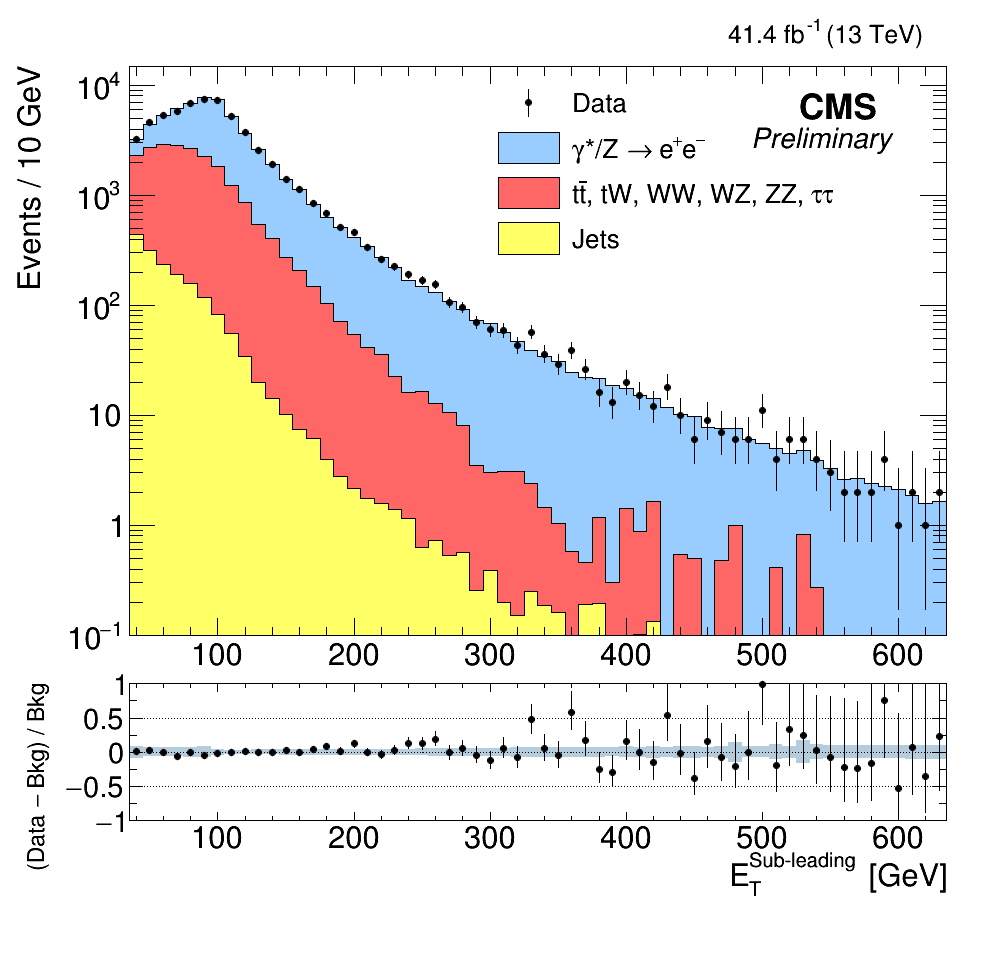
\includegraphics[width=0.32\textwidth]{figures/Zprime/2017/complementary/h_sub_Et.png}&
      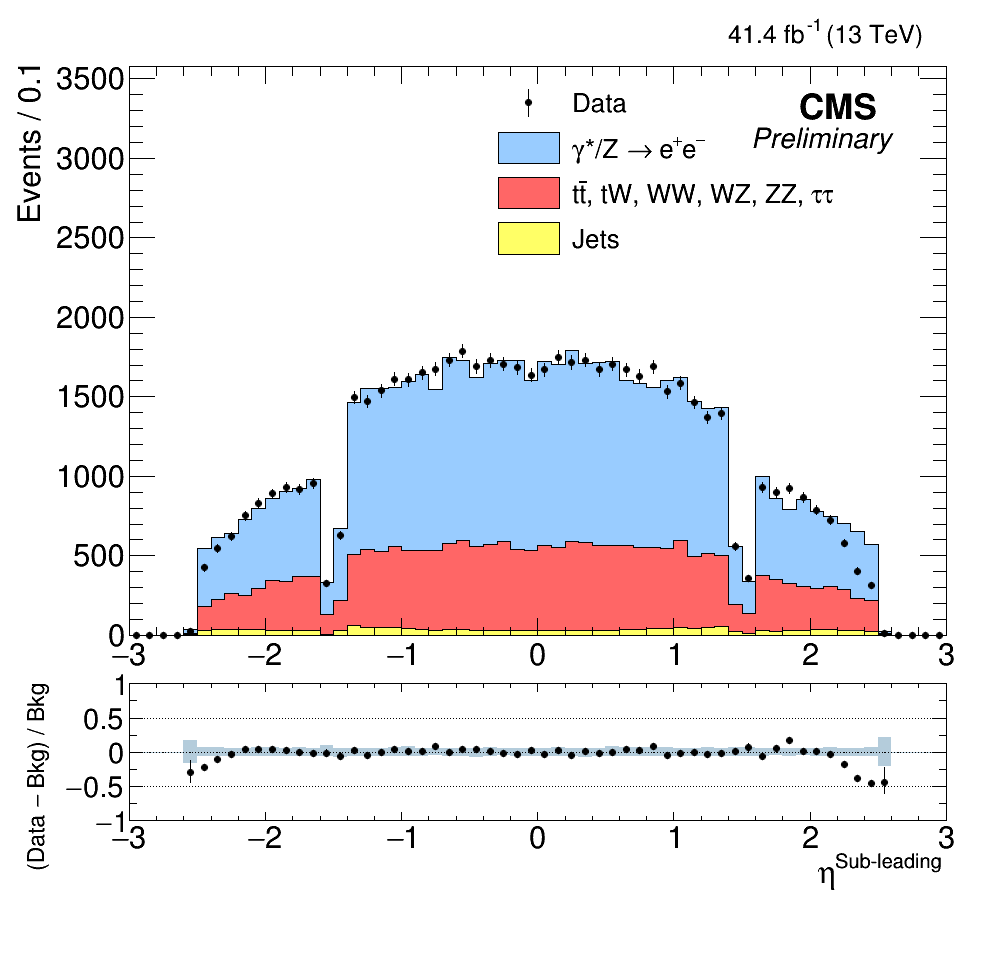
\includegraphics[width=0.32\textwidth]{figures/Zprime/2017/complementary/h_sub_eta.png}&
      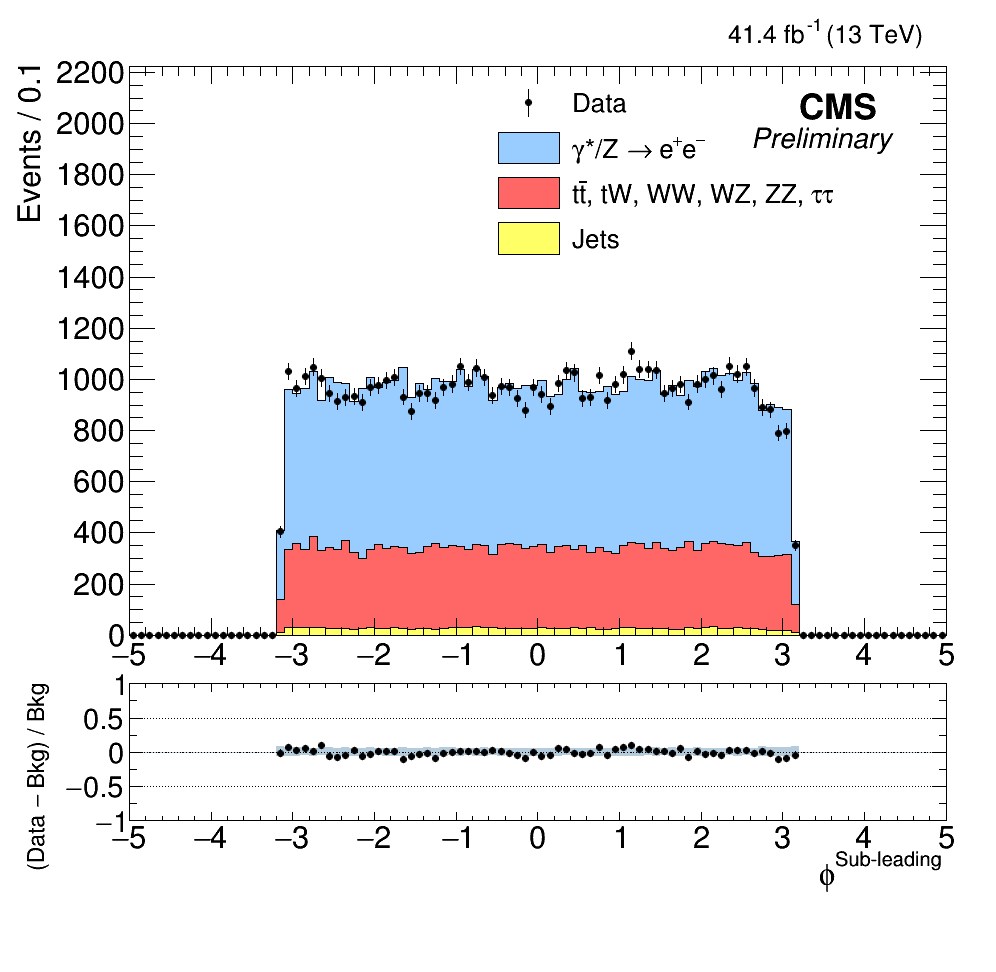
\includegraphics[width=0.32\textwidth]{figures/Zprime/2017/complementary/h_sub_phi.png}\\
      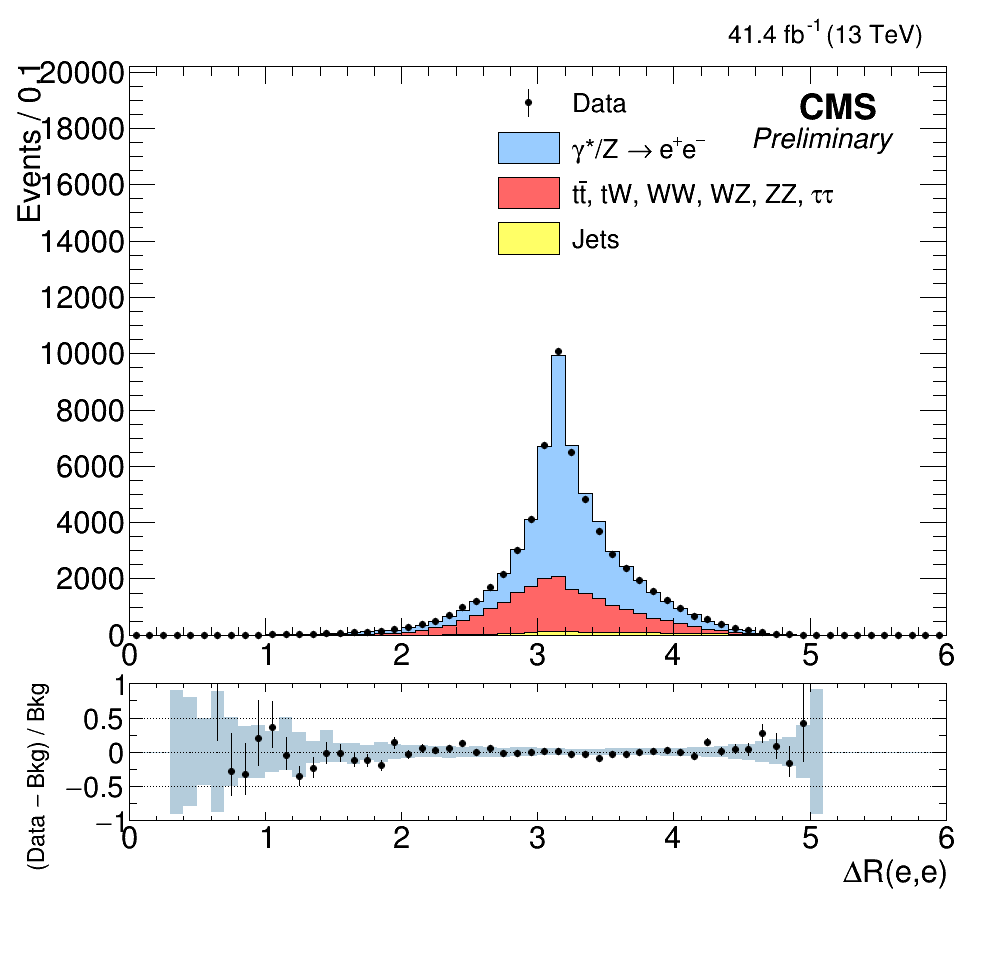
\includegraphics[width=0.32\textwidth]{figures/Zprime/2017/complementary/h_DR_ll.png}&
      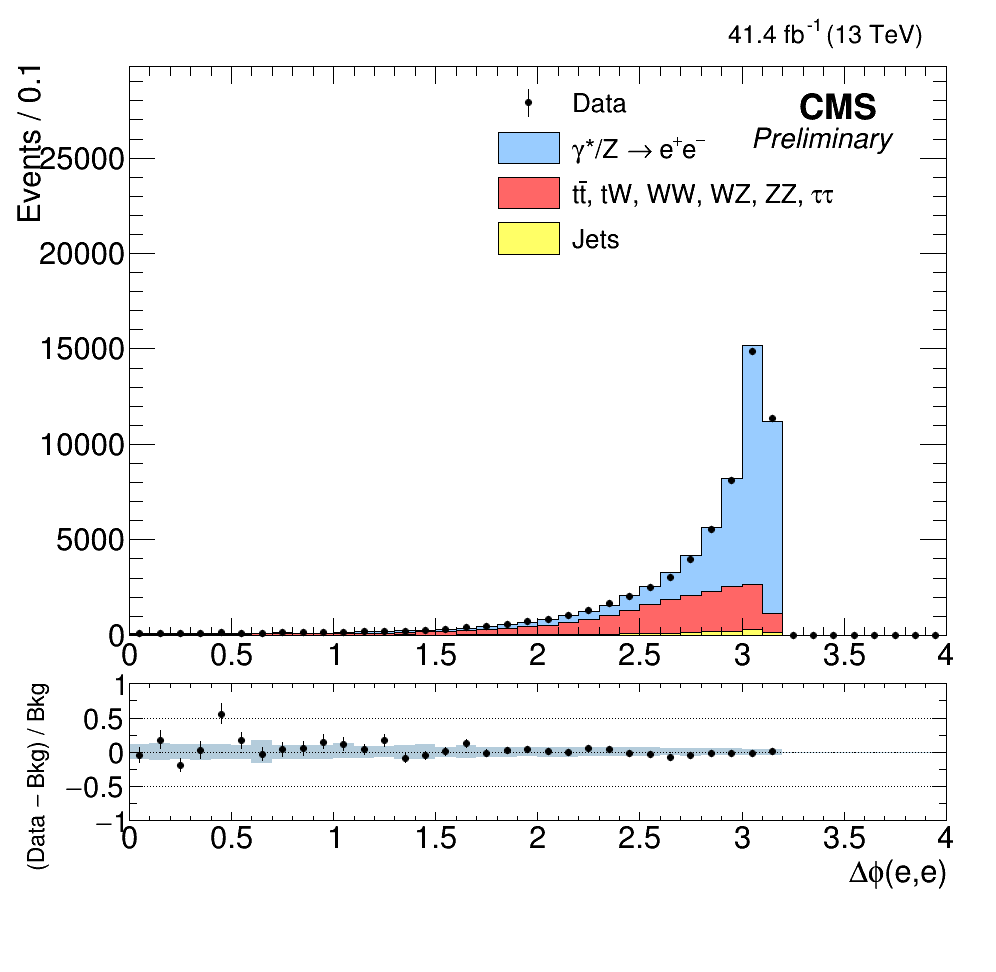
\includegraphics[width=0.32\textwidth]{figures/Zprime/2017/complementary/h_Dphi_ll.png}&
      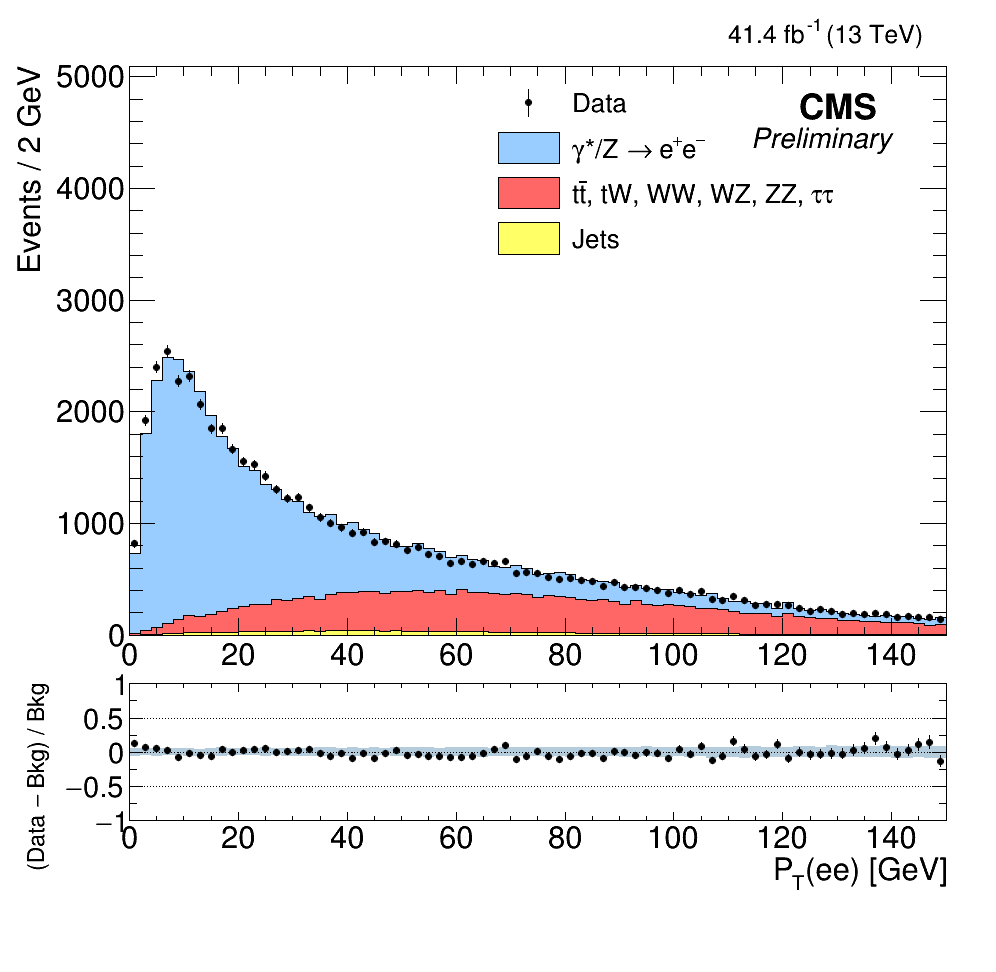
\includegraphics[width=0.32\textwidth]{figures/Zprime/2017/complementary/h_Ptll.png}\\
    \end{tabular}
    \caption{The distributions of invariant mass of two electrons in barrel-barrel, barrel-endcap and barrel-barrel + barrel-endcap (first row), \et, $\eta$ and $\phi$ of leading electron (second row) and \et, $\eta$ and $\phi$ of sub-leading electron (third row),$\Delta R$, $\Delta\phi$ between two electrons and \pt of Z (fourth row) in 2017.
    \label{fig:complementary_2017}}
  \end{center}
\end{figure}


\clearpage

